\documentclass[12pt,a4paper]{article}
% =============================================================================
% Gasto público em educação, salários regionais e dinâmica fiscal no Brasil
% Versão ampliada — painel + DSGE fiscal com capital humano
% Impactos: cenários 1/5/10/25% + teto (EC 95); custo fiscal em R$; efeito
% Laffer da educação; desigualdade regional (Gini/Lorenz/SE-NE); bem-estar;
% multiplicadores; trajetórias de 30 anos.
% =============================================================================
\usepackage[utf8]{inputenc}
\usepackage[T1]{fontenc}
\usepackage[brazil]{babel}
\usepackage{lmodern}
\usepackage{geometry}
\geometry{left=2.5cm,right=2.5cm,top=2.5cm,bottom=2.5cm}
\usepackage{setspace}
\onehalfspacing
\usepackage{graphicx}
\usepackage{float}
\usepackage{booktabs}
\usepackage{longtable}
\usepackage{array}
\usepackage{tabularx}
\usepackage{threeparttable}
\usepackage{caption}
\usepackage{subcaption}
\usepackage{amsmath,amssymb}
\usepackage{siunitx}
\usepackage{enumitem}
\usepackage{xcolor}
\usepackage{multirow}
\usepackage{pdflscape}
\usepackage{ragged2e}
\usepackage[round,authoryear]{natbib}
\bibliographystyle{plainnat}
\usepackage[colorlinks=true,linkcolor=black,citecolor=blue!50!black,urlcolor=blue!50!black]{hyperref}

\renewcommand{\tablename}{Tabela}
\renewcommand{\figurename}{Figura}
\renewcommand{\bibname}{Refer\^encias}
\captionsetup{font=small,labelfont=bf,justification=centering}
\setlist[itemize]{leftmargin=1.2cm}
\setlist[enumerate]{leftmargin=1.2cm}
\newcolumntype{Y}{>{\RaggedRight\arraybackslash}X}
\newcommand{\fonte}[1]{\vspace{0.05cm}\captionsetup{font=scriptsize}\caption*{\footnotesize Fonte: #1}}
\newcommand{\Ee}{\mathbb{E}}

\title{\textbf{Gasto P\'ublico em Educa\c{c}\~ao, Sal\'arios Regionais e Din\^amica Fiscal no Brasil:}\\[2pt]
\textbf{\large Evid\^encias em Painel e um DSGE Fiscal com Capital Humano}}

\author{
Valber Gregory Barbosa Costa Bezerra Santos\thanks{Universidade Federal de Alagoas (UFAL) -- Unidade Educacional de Penedo; Tribunal de Justi\c{c}a do Estado de Alagoas. E-mail: \texttt{valber.santos@penedo.ufal.br}. Para submiss\~ao em avalia\c{c}\~ao \`as cegas, suprimir esta nota de rodap\'e.}
}
\date{\today}

\begin{document}
\maketitle

\begin{center}
\small \textbf{\'Area ANPEC sugerida:} 5 -- Economia do Setor P\'ublico (aderente tamb\'em \`as \'Areas 4 -- Macroeconomia e 10 -- Economia Regional e Urbana). \\
\textbf{Classifica\c{c}\~ao JEL:} E62; H52; I28; J31; O15; R11; C23.
\end{center}

% ------------------------------- RESUMO --------------------------------------
\begin{abstract}
% AUTHOR WRITES
\end{abstract}

\begin{center}\rule{0.6\textwidth}{0.3pt}\end{center}
% AUTHOR WRITES: Abstract

% =============================================================================
\section{Introdu\c{c}\~ao}
% AUTHOR WRITES
% =============================================================================

% =============================================================================
\section{Revis\~ao de literatura}
% AUTHOR WRITES
% =============================================================================
\subsection{Capital humano, educa\c{c}\~ao p\'ublica e crescimento}
% AUTHOR WRITES

\subsection{Da RBC ao DSGE fiscal}
% AUTHOR WRITES

\subsection{Multiplicadores fiscais regionais e DSGE brasileiro}
% AUTHOR WRITES

% =============================================================================
\section{Estrat\'egia emp\'irica}\label{sec:empirica}
% AUTHOR WRITES
% =============================================================================
\subsection{Modelo de efeitos fixos bidirecionais}
% AUTHOR WRITES

\subsection{Endogeneidade e din\^amica}
% AUTHOR WRITES

\subsection{Heterogeneidade regional e encolhimento}
% AUTHOR WRITES

% =============================================================================
\section{Dados e vari\'aveis}\label{sec:dados}
% AUTHOR WRITES
% =============================================================================

\begin{table}[H]
\centering
\caption{Estat\'isticas descritivas (base calibrada, 27 UF $\times$ 13 anos)}
\label{tab:desc}
\small
\begin{tabular}{lrrrr}
\toprule
Variável & Média & Desvio & Mínimo & Máximo \\
\midrule
Salário médio (R\$) & 2.447,1 & 687,8 & 1.323,1 & 4.284,0 \\
Gasto educ. pc (R\$) & 735,8 & 185,9 & 383,1 & 1.736,9 \\
PIB pc (R\$) & 31.099,9 & 6.873,1 & 18.617,0 & 53.144,8 \\
\bottomrule
\end{tabular}

\fonte{Elabora\c{c}\~ao pr\'opria.}
\end{table}

\begin{table}[H]
\centering
\caption{Matriz de correla\c{c}\~ao das vari\'aveis (n\'ivel log)}
\label{tab:corr}
\small
\begin{tabular}{lccc}
\toprule
 & $\log$ Salário & $\log$ Gasto educ. & $\log$ PIB pc \\
\midrule
$\log$ Salário & 1.000 & 0.430 & 0.853 \\
$\log$ Gasto educ. & 0.430 & 1.000 & 0.255 \\
$\log$ PIB pc & 0.853 & 0.255 & 1.000 \\
\bottomrule
\end{tabular}

\fonte{Elabora\c{c}\~ao pr\'opria.}
\end{table}

\begin{figure}[H]
\centering
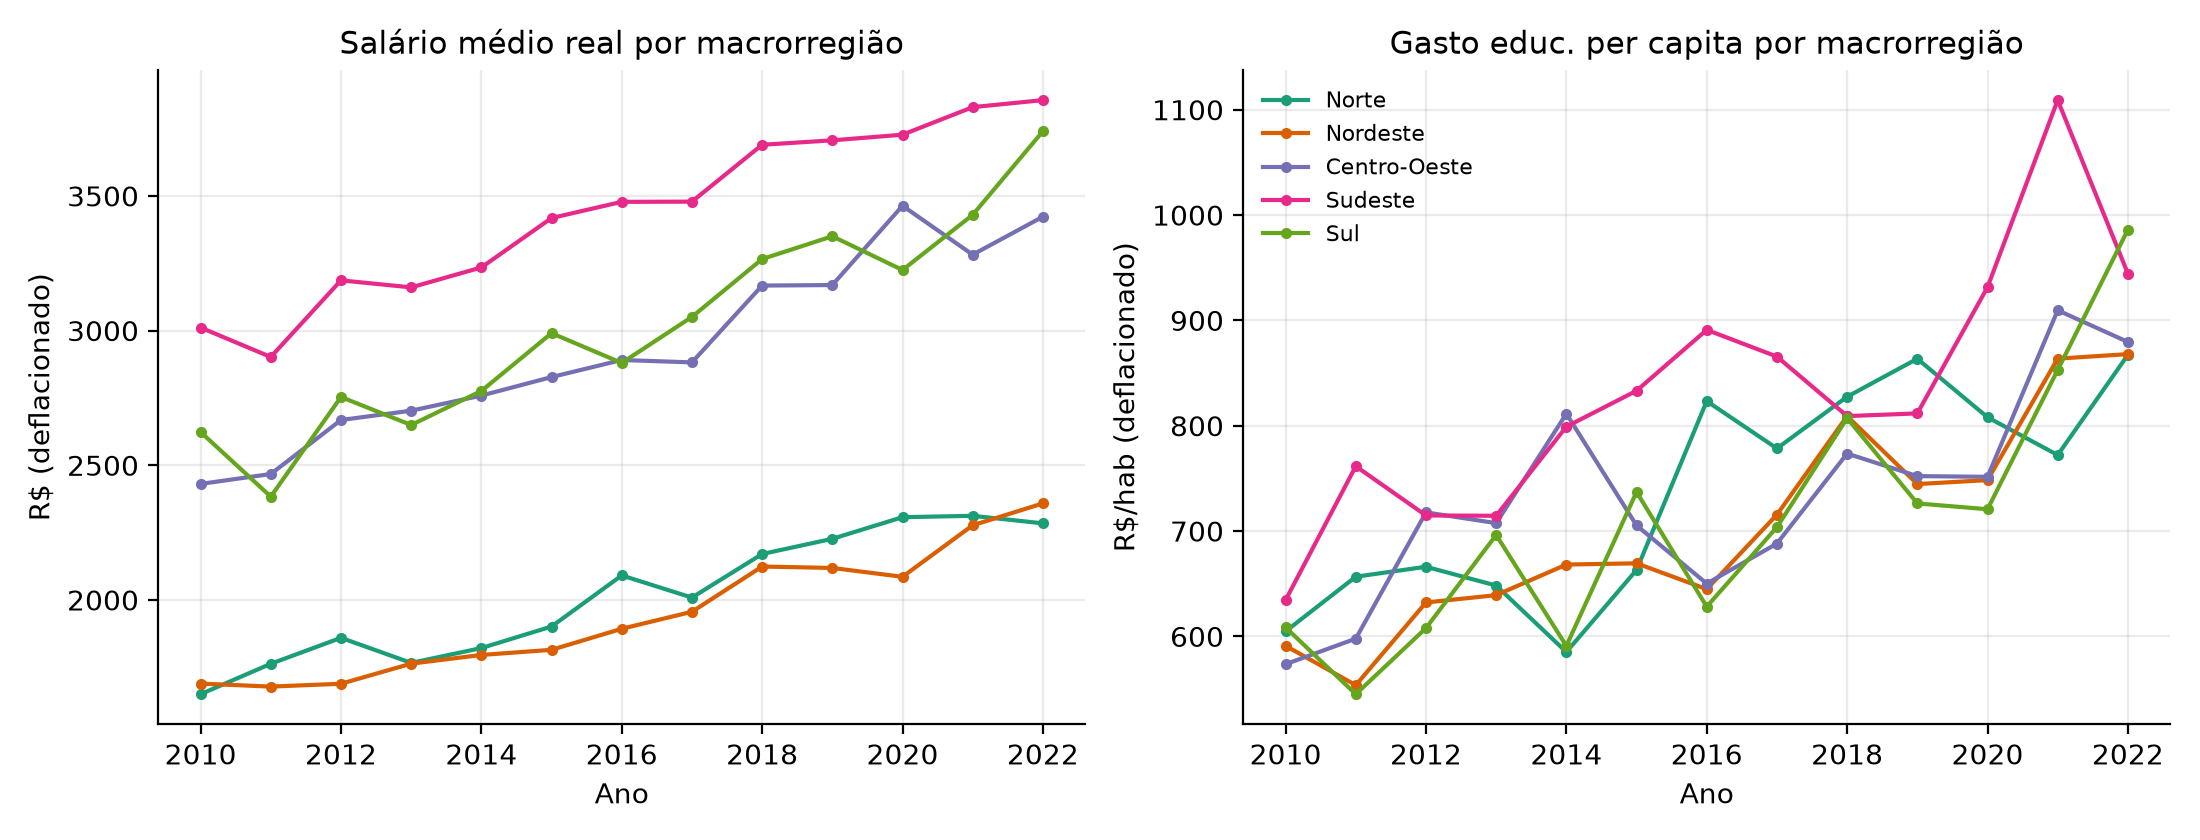
\includegraphics[width=\textwidth]{figures/evolucao_painel.png}
\caption{Evolu\c{c}\~ao do sal\'ario m\'edio real e do gasto educacional per capita por macrorregi\~ao (2010--2022)}
\label{fig:evol}
\fonte{Elabora\c{c}\~ao pr\'opria (base calibrada).}
\end{figure}

% =============================================================================
\section{Resultados emp\'iricos}\label{sec:resultados-emp}
% AUTHOR WRITES
% =============================================================================
\subsection{Elasticidade m\'edia}
% AUTHOR WRITES

\begin{table}[H]
\centering
\caption{Modelo de efeitos fixos -- vari\'avel dependente: $\log$(sal\'ario m\'edio)}
\label{tab:fe}
\small
\begin{tabular}{lcccc}
\toprule
 & (1) Pooled & (2) FE 2-vias & (3) FE 2-vias & (4) FE entidade \\
 & OLS & Clustered & Driscoll-Kraay & + tendência \\
\midrule
$\log$(Gasto educ. pc) & 0.256*** & 0.173*** & 0.173*** & 0.175*** \\
 & (0.075) & (0.027) & (0.015) & (0.026) \\
$\log$(PIB pc) & 1.021*** & 0.387*** & 0.387*** & 0.411*** \\
 & (0.078) & (0.056) & (0.039) & (0.051) \\
\midrule
Efeitos fixos UF & Não & Sim & Sim & Sim \\
Efeitos fixos ano & Não & Sim & Sim & Não \\
Observações & 351 & 351 & 351 & 351 \\
$R^2$ (within) & -- & 0.603 & 0.603 & 0.833 \\
\bottomrule
\end{tabular}

\begin{minipage}{0.95\textwidth}\vspace{2pt}\scriptsize
Nota: erros-padr\~ao entre par\^enteses. \textsuperscript{*}$p<0{,}10$; \textsuperscript{**}$p<0{,}05$; \textsuperscript{***}$p<0{,}01$. (1) \emph{pooled} OLS; (2) FE bidirecional com erros clusterizados por UF; (3) FE bidirecional com erros de Driscoll--Kraay; (4) FE de entidade com tend\^encia linear.
\end{minipage}
\fonte{Elabora\c{c}\~ao pr\'opria.}
\end{table}

\subsection{Heterogeneidade regional e encolhimento}
% AUTHOR WRITES

\begin{table}[H]
\centering
\caption{Elasticidade sal\'ario-educa\c{c}\~ao por macrorregi\~ao (FE por regi\~ao)}
\label{tab:regiao}
\small
\begin{tabular}{lcccc}
\toprule
Macrorregião & Elasticidade & Erro-padrão & $p$-valor & $N$ \\
\midrule
Norte & 0.206*** & 0.038 & 0.000 & 91 \\
Nordeste & 0.208*** & 0.056 & 0.000 & 117 \\
Centro-Oeste & 0.188*** & 0.039 & 0.000 & 52 \\
Sudeste & -0.009 & 0.086 & 0.919 & 52 \\
Sul & 0.155*** & 0.009 & 0.000 & 39 \\
\bottomrule
\end{tabular}

\begin{minipage}{0.8\textwidth}\vspace{2pt}\scriptsize
Nota: cada linha \'e uma regress\~ao FE separada, com erros clusterizados. \textsuperscript{***}$p<0{,}01$; \textsuperscript{**}$p<0{,}05$.
\end{minipage}
\fonte{Elabora\c{c}\~ao pr\'opria.}
\end{table}

\begin{figure}[H]
\centering
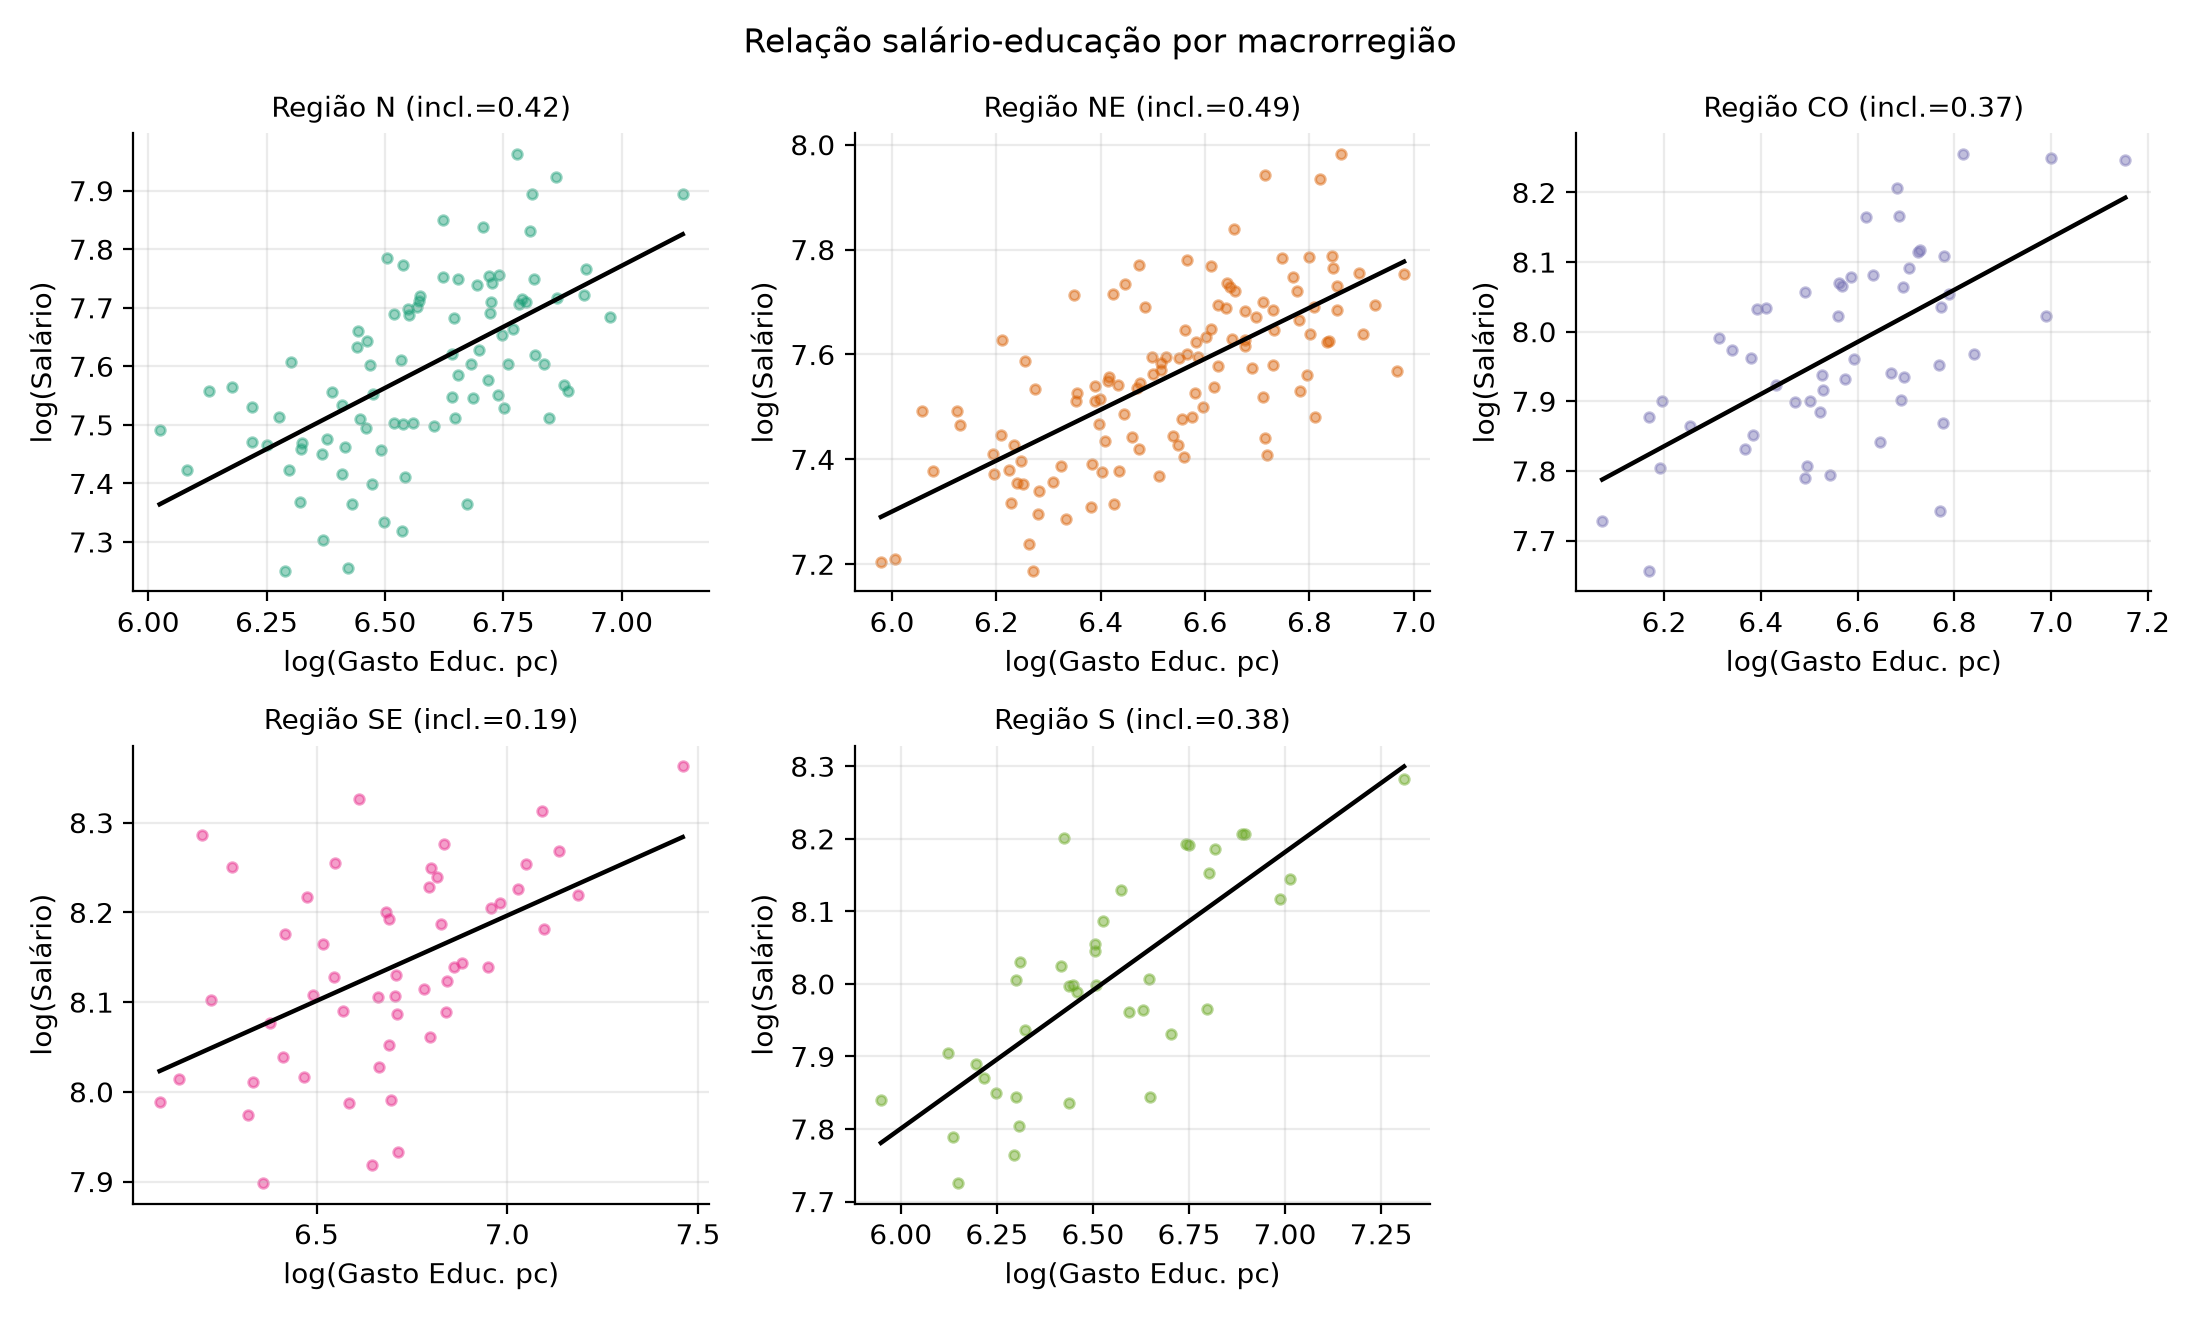
\includegraphics[width=0.93\textwidth]{figures/dispersao_uf.png}
\caption{Rela\c{c}\~ao sal\'ario-educa\c{c}\~ao por macrorregi\~ao}
\label{fig:disp}
\fonte{Elabora\c{c}\~ao pr\'opria.}
\end{figure}

\begin{figure}[H]
\centering
\begin{minipage}{0.49\textwidth}\centering
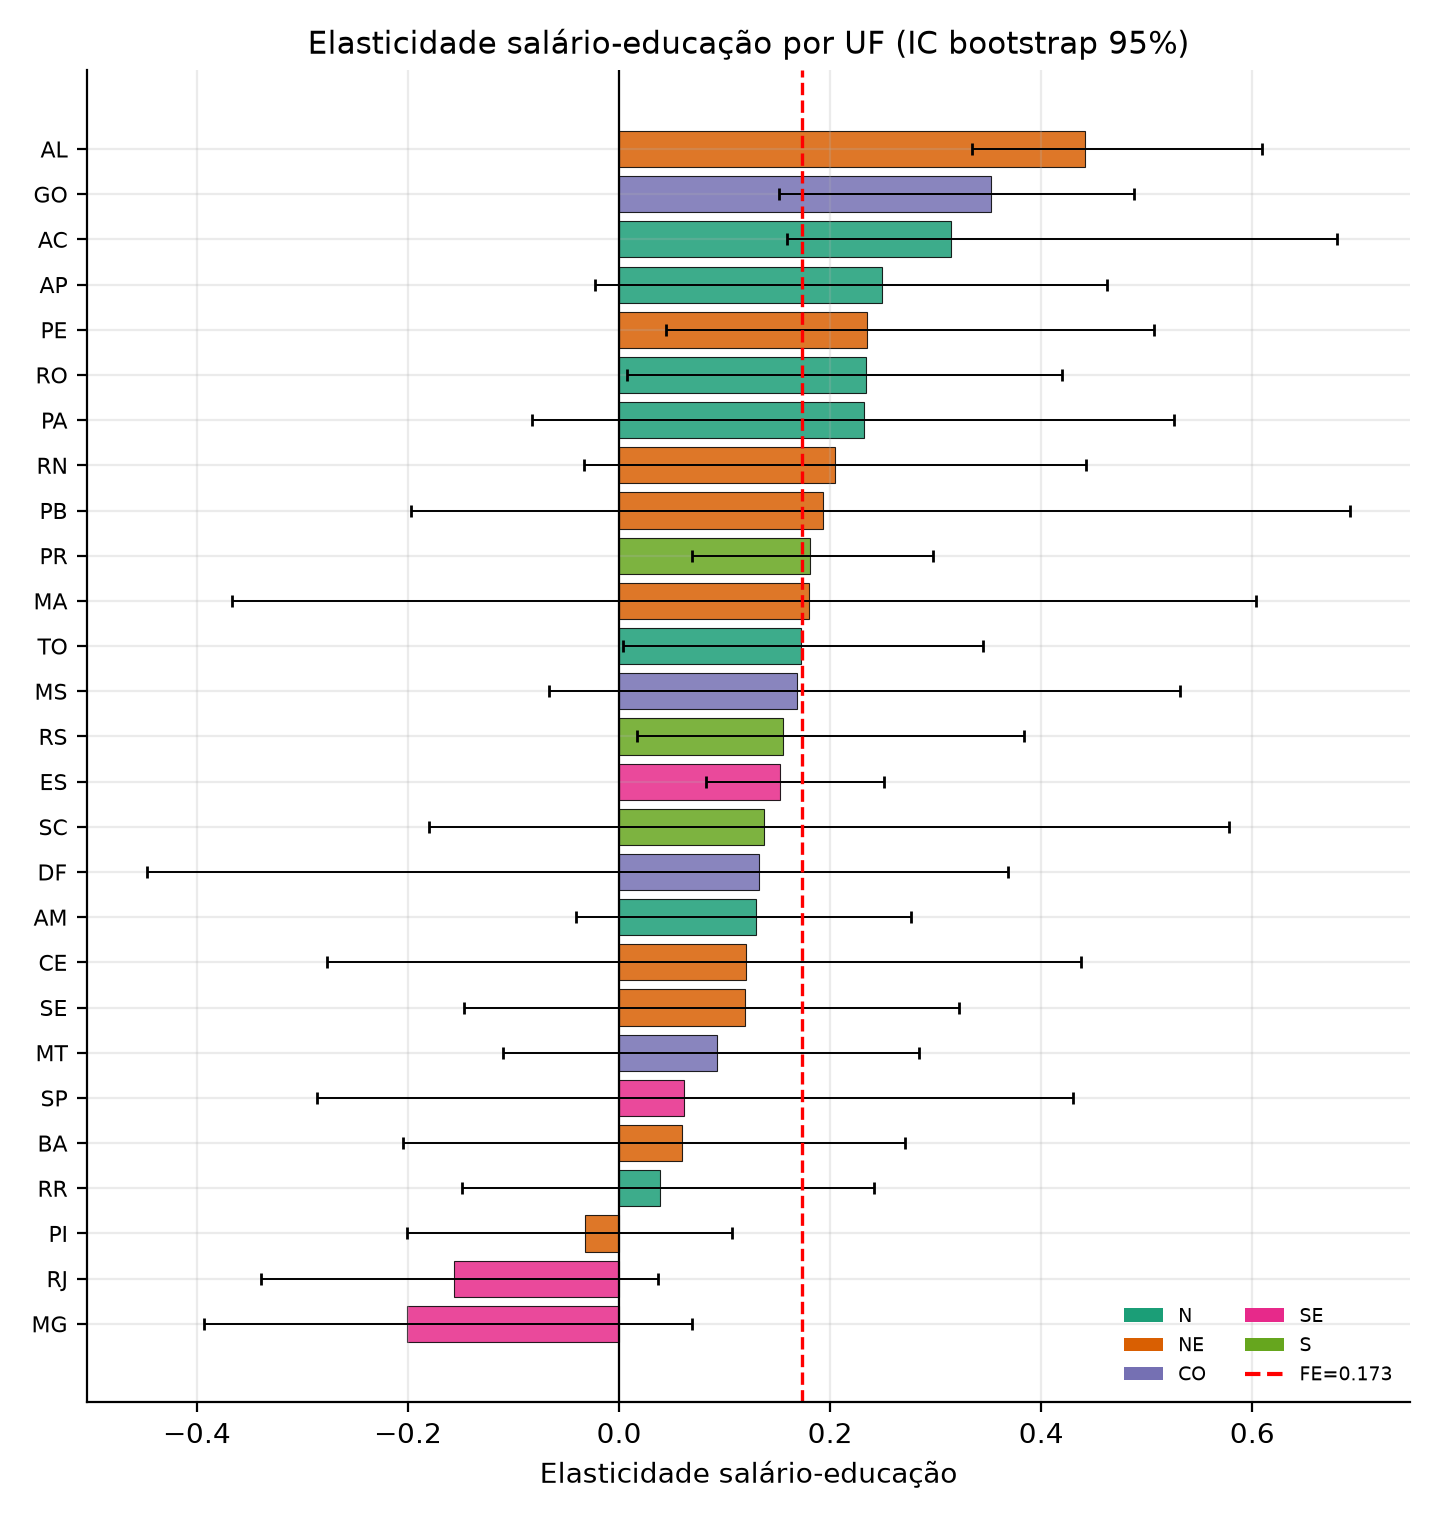
\includegraphics[width=\textwidth]{figures/elasticidade_uf_ic.png}
\end{minipage}\hfill
\begin{minipage}{0.49\textwidth}\centering
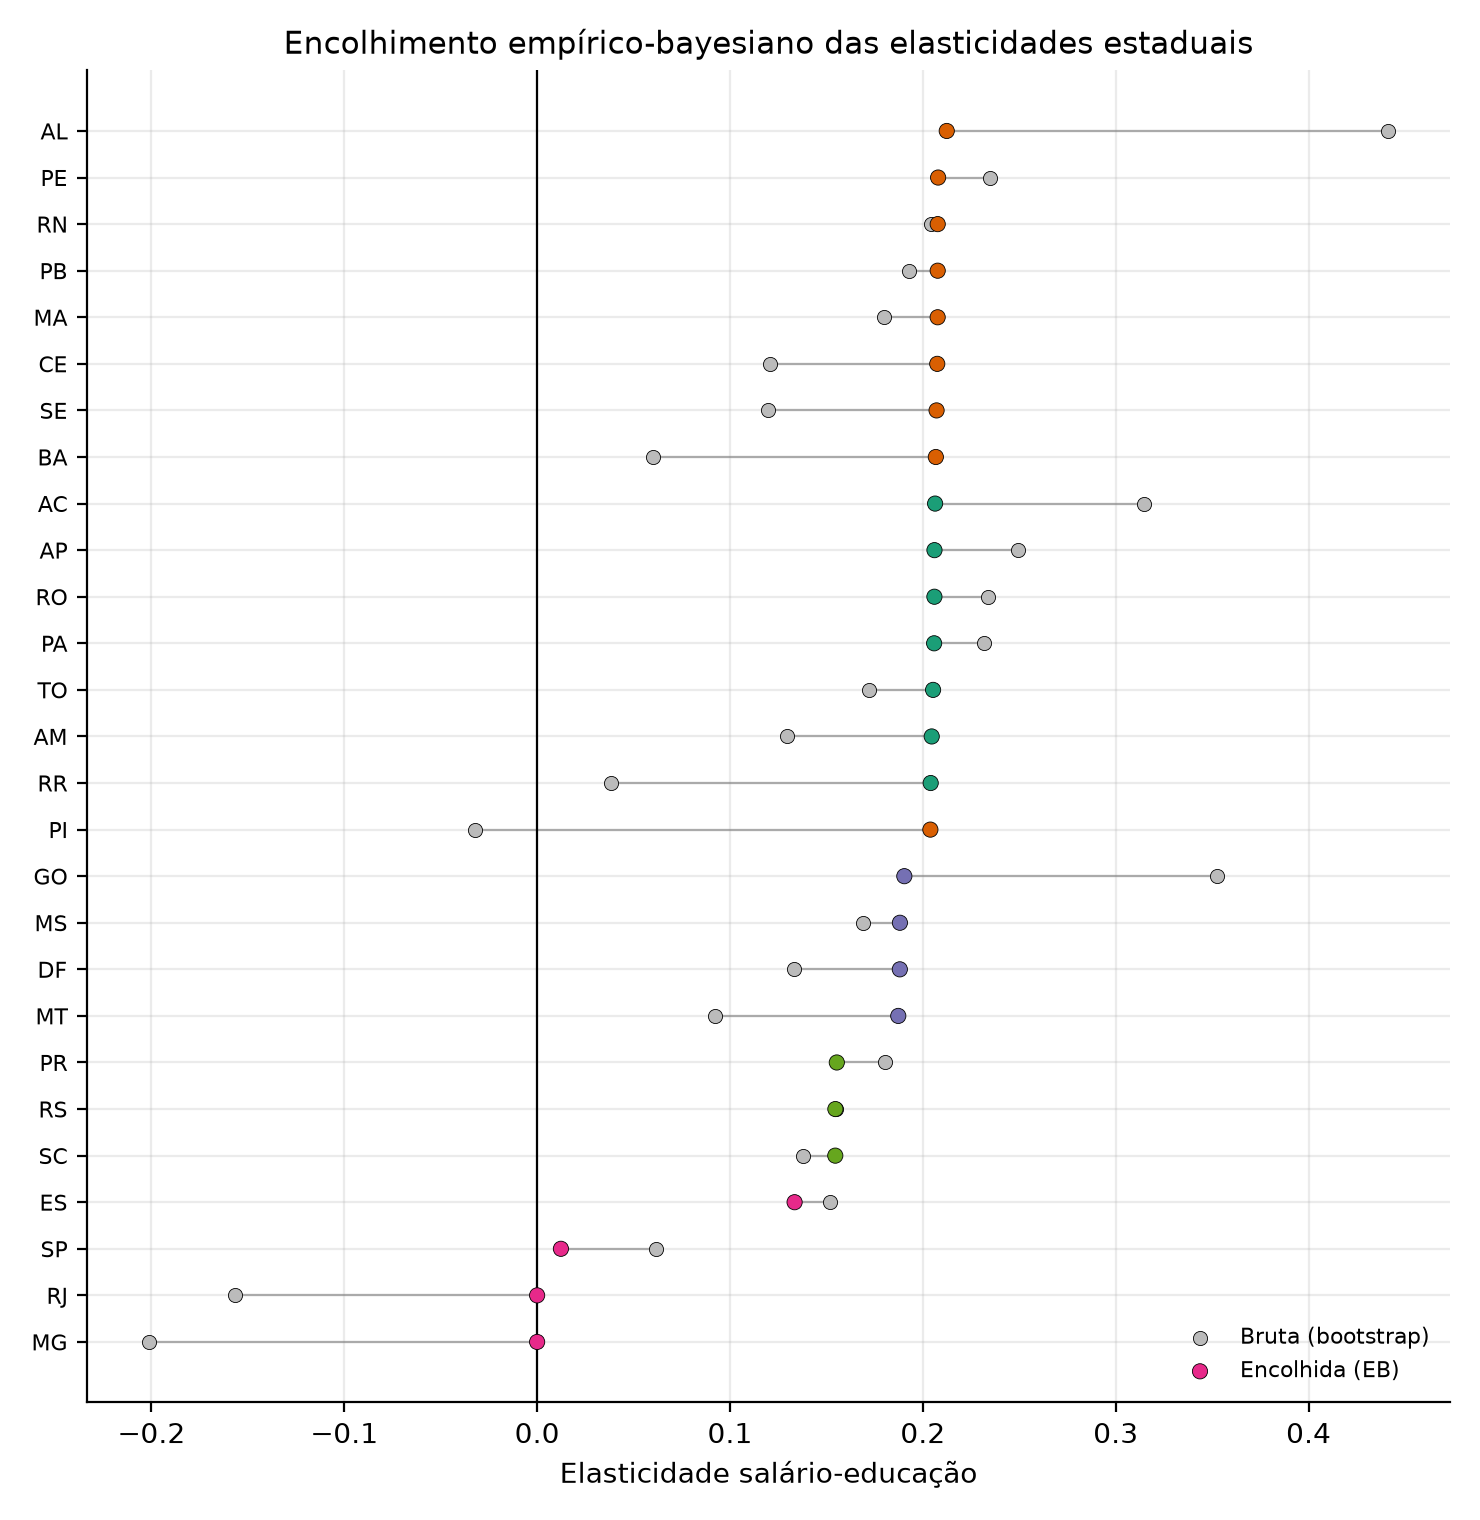
\includegraphics[width=\textwidth]{figures/encolhimento_eb.png}
\end{minipage}
\caption{Elasticidades estaduais com IC \emph{bootstrap} de $95\%$ (esq.) e encolhimento emp\'irico-bayesiano das elasticidades brutas em dire\c{c}\~ao \`as regionais (dir.)}
\label{fig:eb}
\fonte{Elabora\c{c}\~ao pr\'opria a partir de 2.000 reamostragens.}
\end{figure}

\begin{figure}[H]
\centering
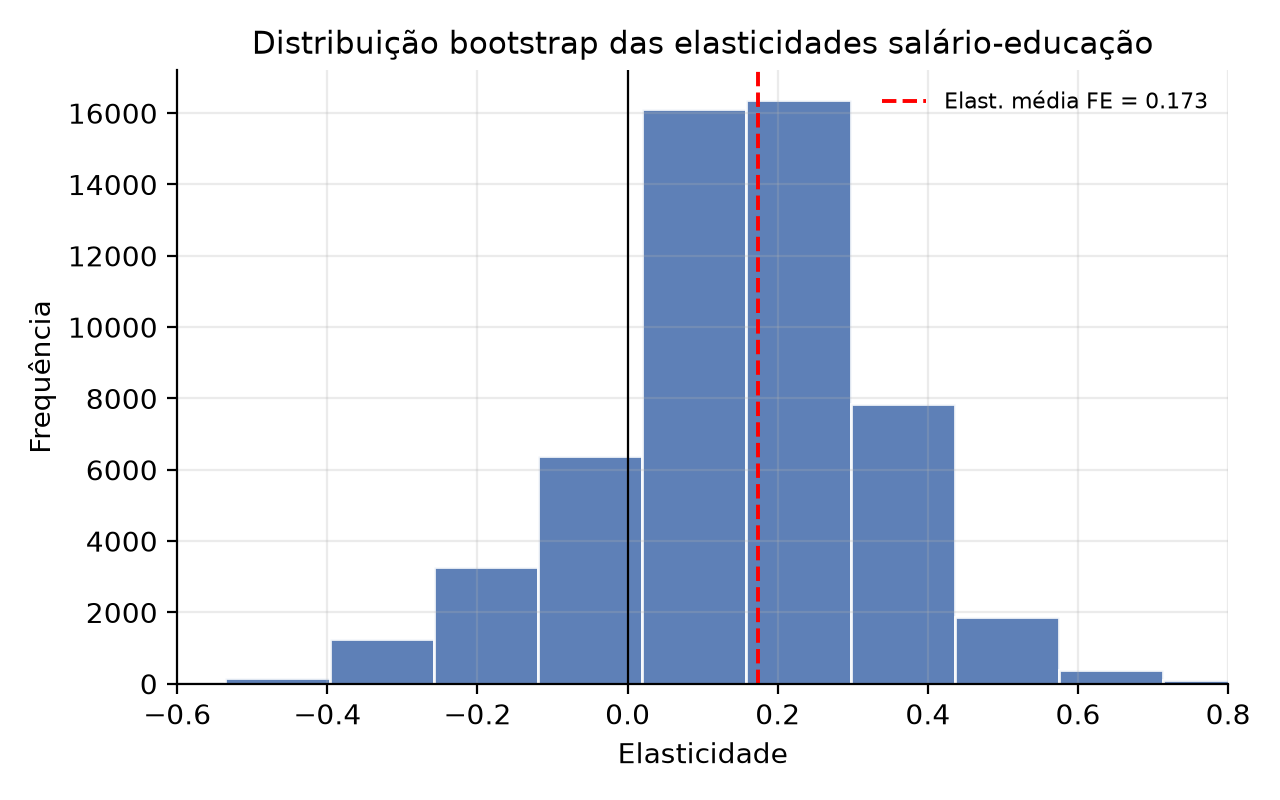
\includegraphics[width=0.62\textwidth]{figures/hist_elasticidades.png}
\caption{Distribui\c{c}\~ao \emph{bootstrap} agregada das elasticidades sal\'ario-educa\c{c}\~ao}
\label{fig:hist}
\fonte{Elabora\c{c}\~ao pr\'opria.}
\end{figure}

% =============================================================================
\section{O modelo DSGE fiscal com capital humano}\label{sec:dsge}
% AUTHOR WRITES
% =============================================================================

\subsection{Fam\'ilias, firmas e capital humano}
% AUTHOR WRITES

\begin{table}[H]
\centering
\caption{Calibra\c{c}\~ao do modelo DSGE}
\label{tab:dsgepar}
\small
\begin{tabular}{cll}
\toprule
Parâmetro & Valor & Interpretação \\
\midrule
$\alpha$ & 0,40 & Participação do capital físico na produção \\
$\beta$ & 0,96 & Fator de desconto intertemporal (anual) \\
$\delta_k$ & 0,10 & Depreciação do capital físico \\
$\delta_h$ & 0,04 & Depreciação do capital humano \\
$\tau$ & 0,33 & Carga tributária efetiva (\% do PIB) \\
$\theta$ & 1,75 & Peso do lazer na utilidade \\
$\phi$ & 0,30 & Elasticidade do capital humano ao gasto público \\
$g_e$ & 0,05 & Gasto público em educação / PIB no EE \\
$\rho_G$ & 0,90 & Persistência do choque fiscal (transitório) \\
$A$ & 0,134 & Produtividade da tecnologia educacional (calibrada) \\
\bottomrule
\end{tabular}

\begin{minipage}{0.9\textwidth}\vspace{2pt}\scriptsize
Nota: refer\^encia \`a literatura DSGE brasileira \citep{castro2015samba,cavalcantivereda2015}. $\tau=0{,}33$ reflete a carga/PIB; $\phi=0{,}30$ situa-se na faixa das estimativas de produtividade do gasto p\'ublico produtivo \citep{bomligthart2014}.
\end{minipage}
\fonte{Elabora\c{c}\~ao pr\'opria.}
\end{table}

\subsection{M\'etodo de solu\c{c}\~ao}
% AUTHOR WRITES

% =============================================================================
\section{Resultados do DSGE: o preju\'izo de cortar educa\c{c}\~ao}\label{sec:resultados-dsge}
% AUTHOR WRITES
% =============================================================================
\subsection{Fun\c{c}\~oes impulso-resposta}
% AUTHOR WRITES

\begin{figure}[H]
\centering
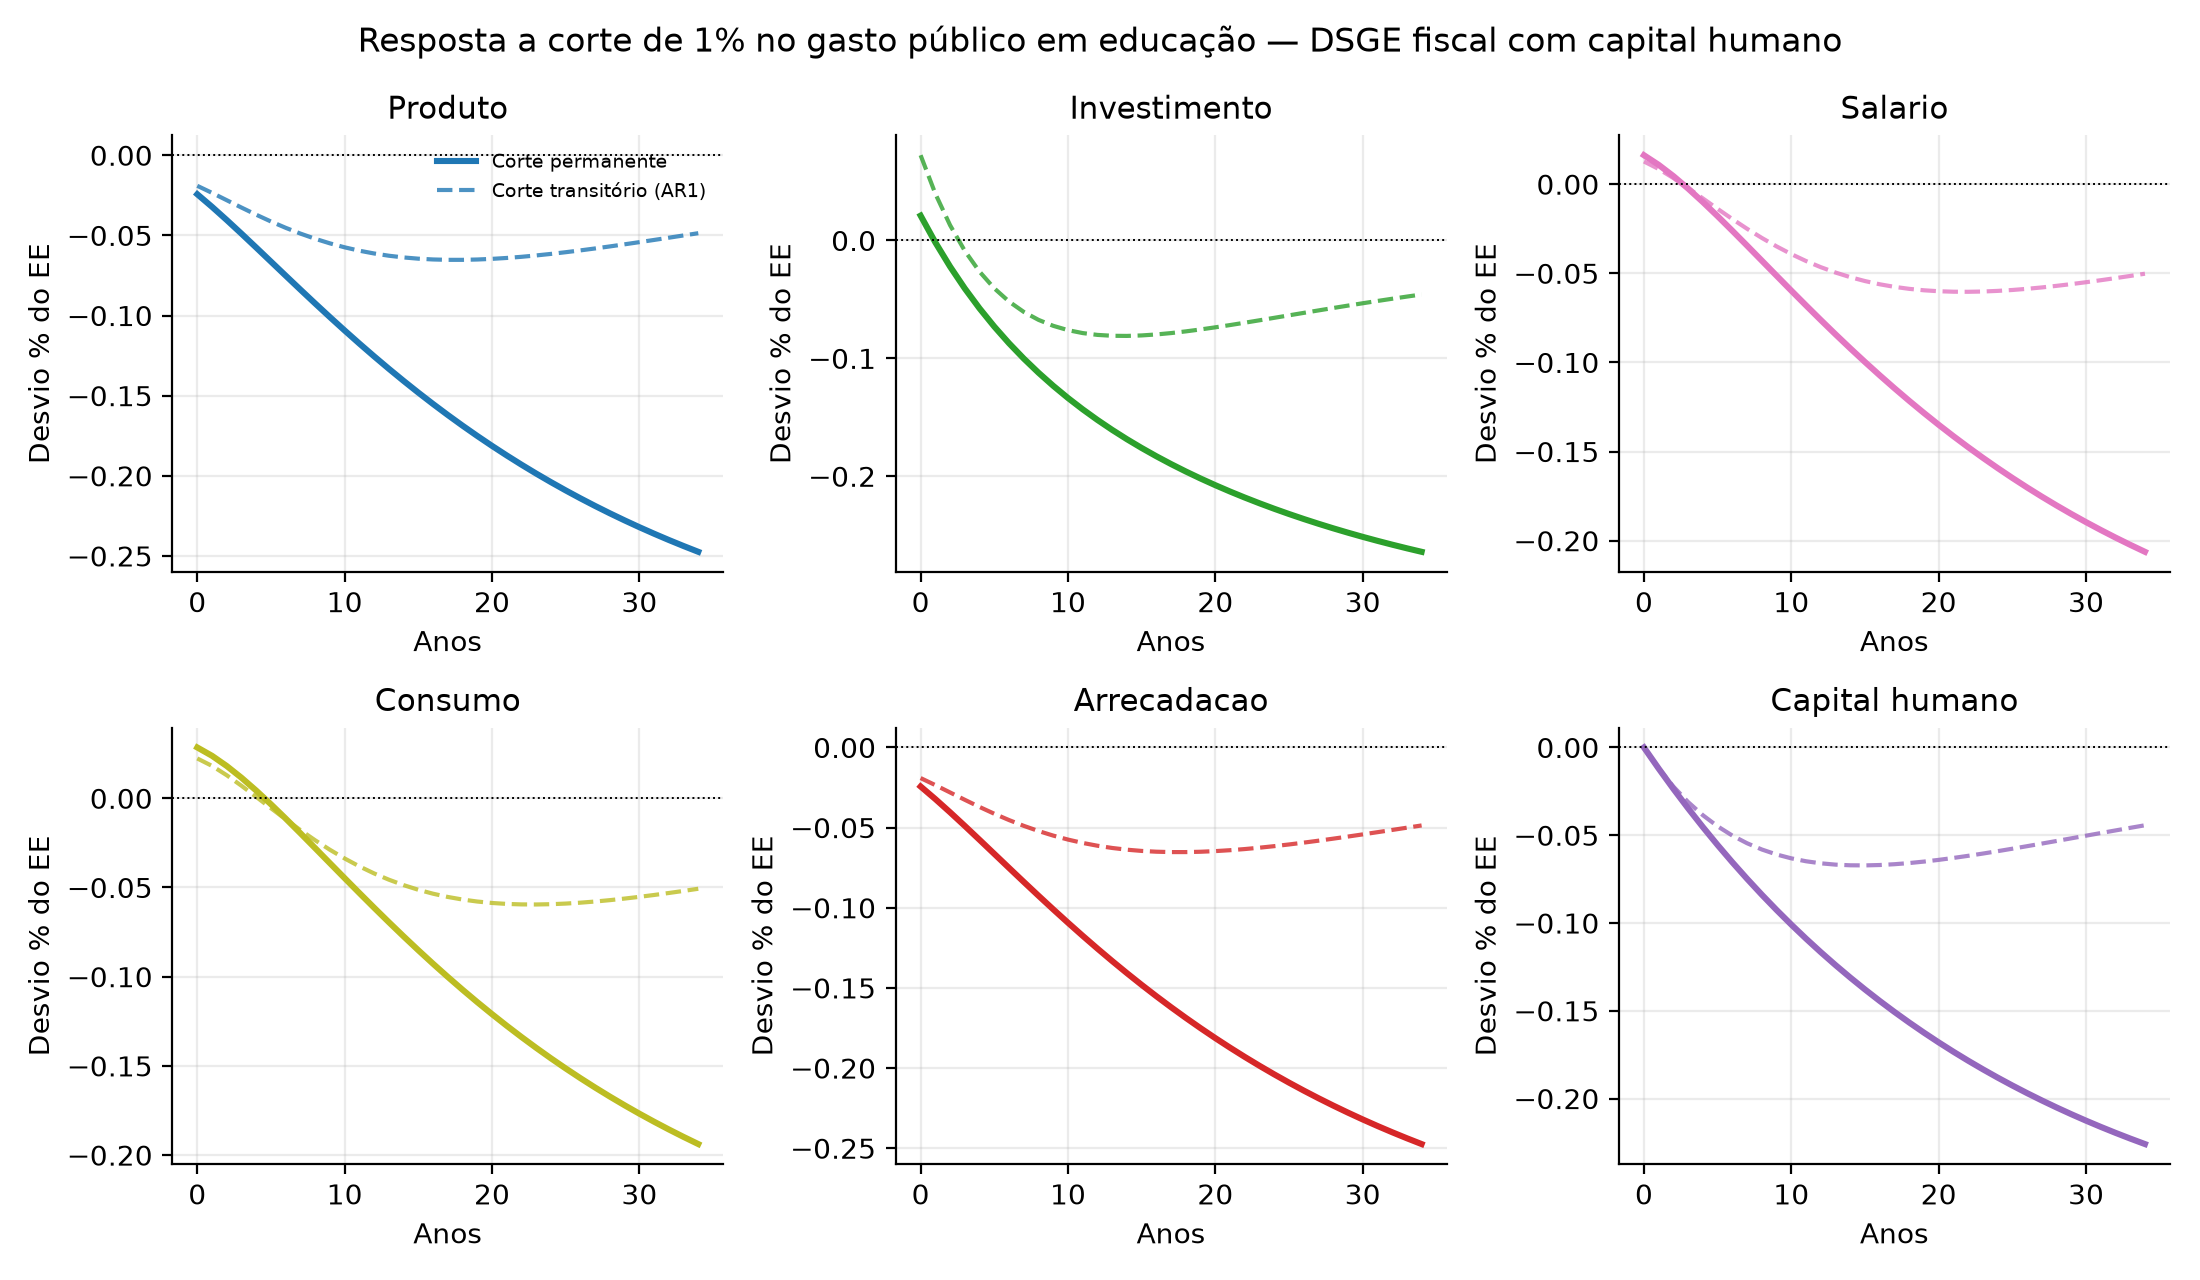
\includegraphics[width=\textwidth]{figures/irf_corte_educacao.png}
\caption{Resposta a corte de $1\%$ no gasto p\'ublico em educa\c{c}\~ao: permanente (linha cheia) e transit\'orio (tracejada)}
\label{fig:irf}
\fonte{Simula\c{c}\~ao DSGE por previs\~ao perfeita n\~ao linear.}
\end{figure}

\begin{table}[H]
\centering
\caption{Resposta ao corte permanente de $1\%$ (desvios \% do EE e perdas acumuladas descontadas)}
\label{tab:irf}
\small
\begin{tabular}{lrrrr}
\toprule
Variável & Impacto (t=0) & 5 anos & Perda acum. 10a & Perda acum. 20a \\
\midrule
Produto & -0,024 & -0,066 & 0,497 & 1,283 \\
Investimento & 0,021 & -0,073 & 0,455 & 1,391 \\
Salario & 0,016 & -0,018 & 0,108 & 0,623 \\
Consumo & 0,028 & -0,003 & -0,010 & 0,424 \\
Arrecadacao & -0,024 & -0,066 & 0,497 & 1,283 \\
\bottomrule
\end{tabular}

\begin{minipage}{0.9\textwidth}\vspace{2pt}\scriptsize
Nota: ``Perda acum.'' \'e a soma descontada (fator $0{,}96$) dos desvios no horizonte, em pontos percentuais-ano. A arrecada\c{c}\~ao acompanha o produto pois $T_t=\tau Y_t$.
\end{minipage}
\fonte{Elabora\c{c}\~ao pr\'opria.}
\end{table}

\subsection{Escala do corte: de $1\%$ a $25\%$ e o teto de gasto}
% AUTHOR WRITES

\begin{figure}[H]
\centering
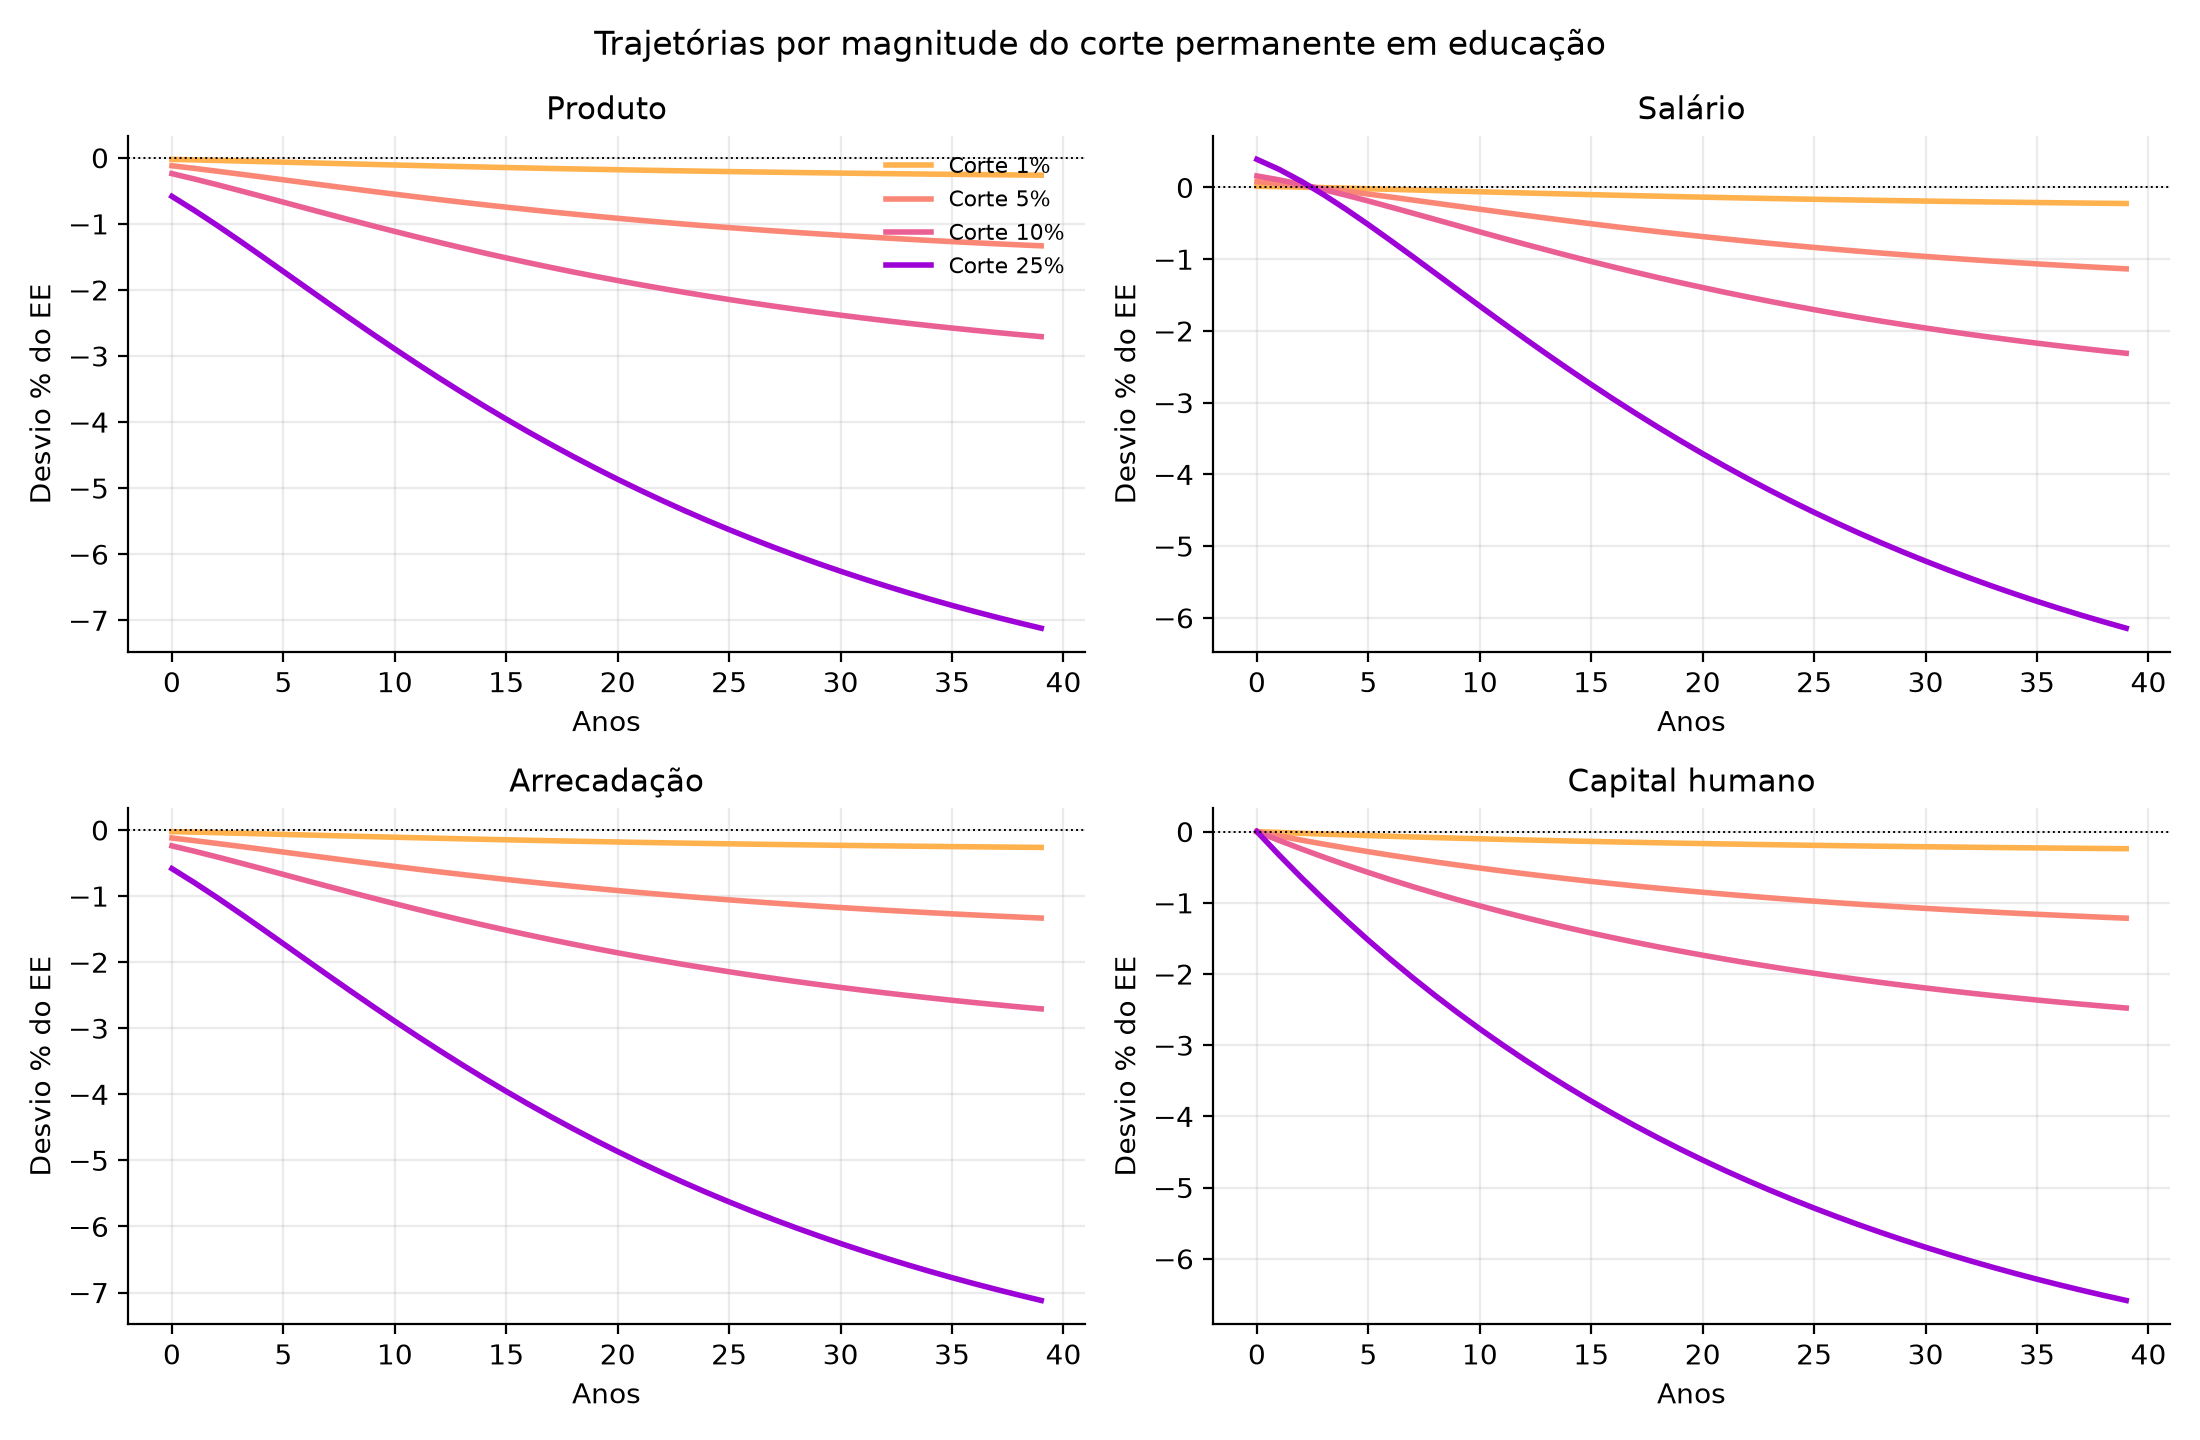
\includegraphics[width=\textwidth]{figures/irf_multi_corte.png}
\caption{Trajet\'orias de produto, sal\'ario, arrecada\c{c}\~ao e capital humano por magnitude do corte permanente}
\label{fig:multi}
\fonte{Simula\c{c}\~ao DSGE.}
\end{figure}

\begin{table}[H]
\centering
\caption{Cen\'arios de corte: efeitos de longo prazo, bem-estar e multiplicador}
\label{tab:cenarios}
\small
\begin{tabular}{lrrrrrr}
\toprule
Corte & $\Delta H_{LP}$ & $\Delta Y_{LP}$ & $\Delta S_{LP}$ & $\Delta T_{LP}$ & Bem-estar & Mult.\ cum.\ 10a \\
 & (\%) & (\%) & (\%) & (\%) & (\% cons.) & \\
\midrule
1\% & -0,301 & -0,334 & -0,301 & -0,334 & 0,084 & 1,19 \\
5\% & -1,527 & -1,693 & -1,527 & -1,693 & 0,428 & 1,19 \\
10\% & -3,111 & -3,440 & -3,111 & -3,440 & 0,884 & 1,20 \\
25\% & -8,267 & -9,066 & -8,266 & -9,066 & 2,445 & 1,23 \\
\bottomrule
\end{tabular}

\begin{minipage}{0.92\textwidth}\vspace{2pt}\scriptsize
Nota: $\Delta X_{LP}$ \'e o desvio percentual de longo prazo (novo EE). Bem-estar em equivalente de consumo permanente (perda \%). Multiplicador acumulado de 10 anos = raz\~ao entre valores presentes de $\Delta Y$ e $\Delta G^e$.
\end{minipage}
\fonte{Elabora\c{c}\~ao pr\'opria.}
\end{table}

\begin{figure}[H]
\centering
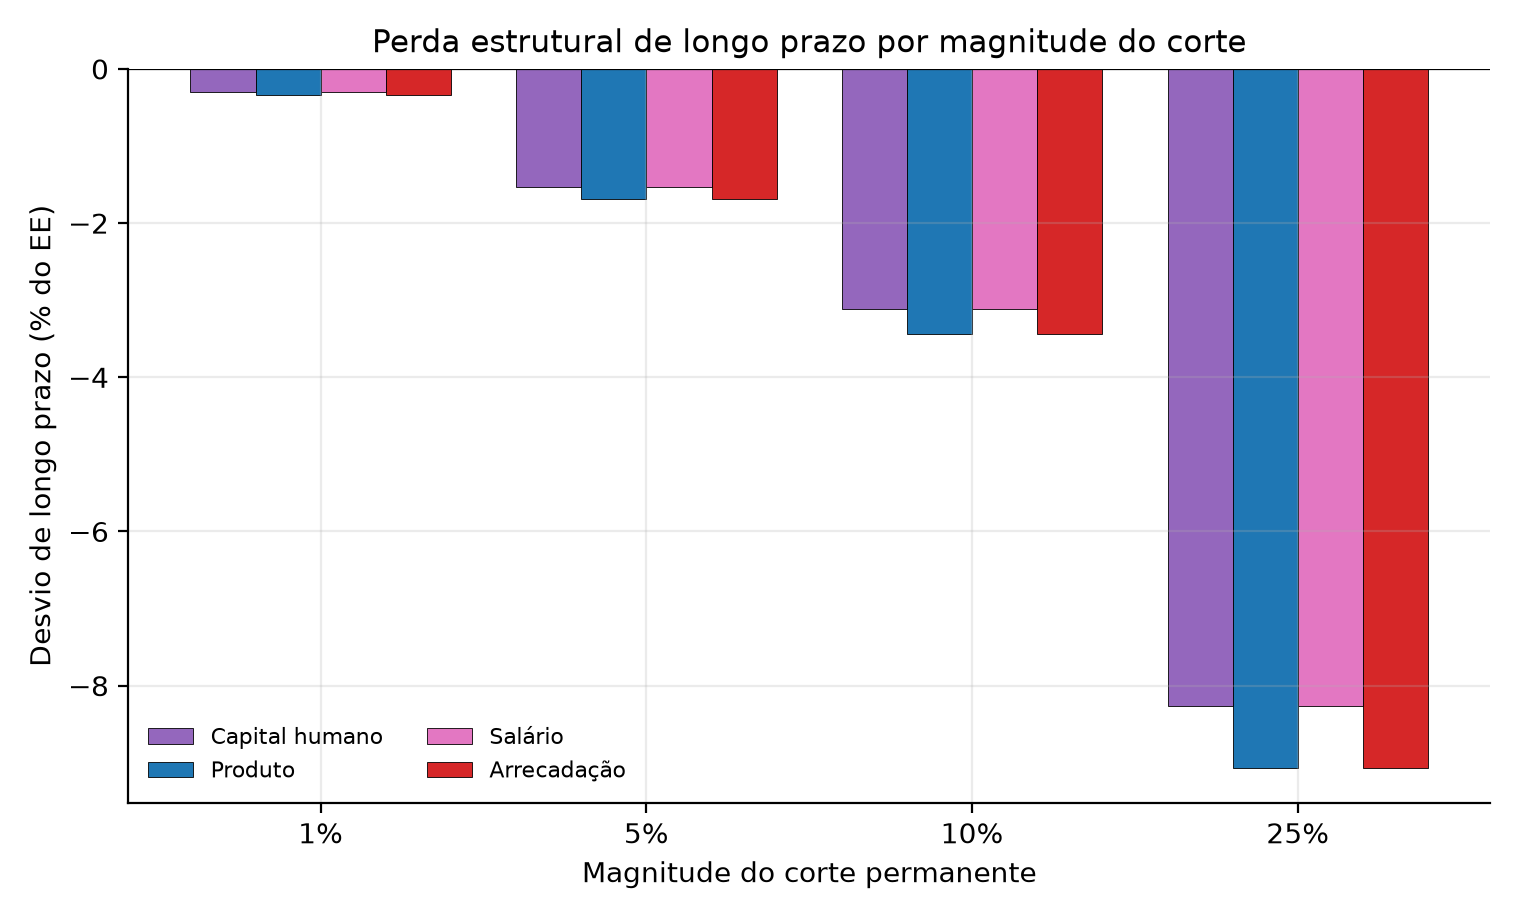
\includegraphics[width=0.8\textwidth]{figures/perdas_por_corte.png}
\caption{Perda estrutural de longo prazo por magnitude do corte permanente}
\label{fig:perdas}
\fonte{Elabora\c{c}\~ao pr\'opria.}
\end{figure}

\begin{figure}[H]
\centering
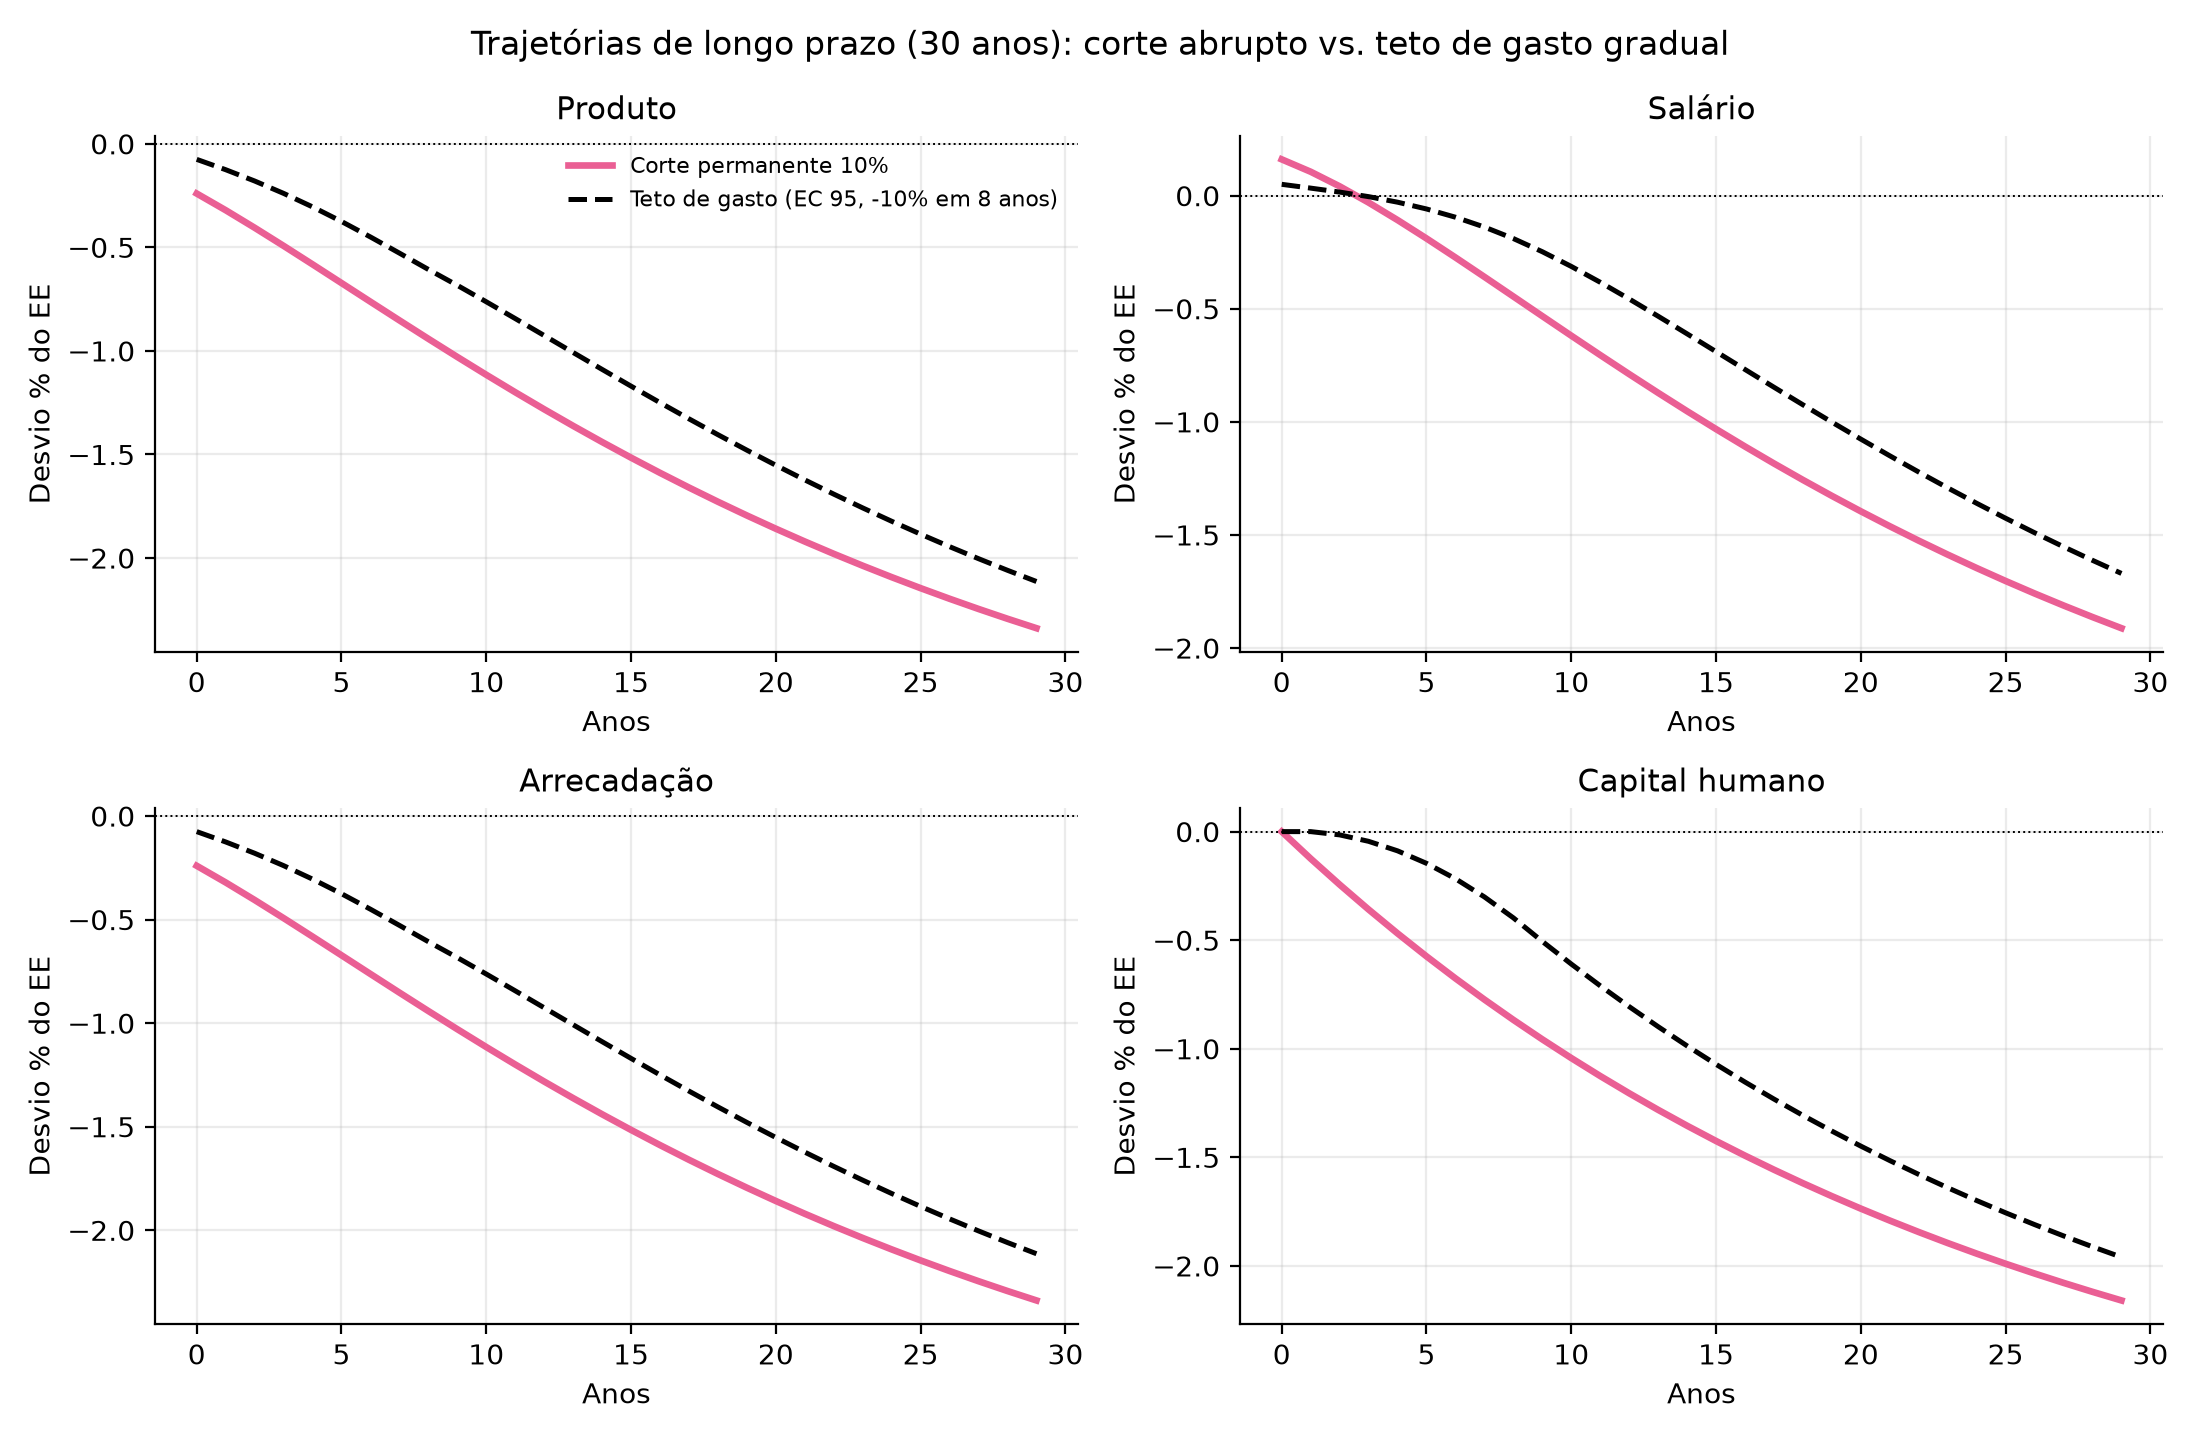
\includegraphics[width=\textwidth]{figures/trajetoria_30anos.png}
\caption{Trajet\'orias de 30 anos: corte abrupto de $10\%$ vs.\ teto de gasto gradual (EC 95)}
\label{fig:traj30}
\fonte{Elabora\c{c}\~ao pr\'opria.}
\end{figure}

% =============================================================================
\section{Custo fiscal l\'iquido: o efeito Laffer din\^amico da educa\c{c}\~ao}\label{sec:laffer}
% AUTHOR WRITES
% =============================================================================

\begin{table}[H]
\centering
\caption{Custo fiscal do corte em educa\c{c}\~ao (valor presente, R\$ bilh\~oes)}
\label{tab:fiscal}
\small
\begin{tabular}{lrrrrr}
\toprule
Corte & Horizonte & Economia (VP) & Perda arrec.\ (VP) & Líquido (VP) & \% erodido \\
 & (anos) & R\$ bi & R\$ bi & R\$ bi & \\
\midrule
1\% & 10 & 45,7 & 17,9 & 27,8 & 39,2\% \\
1\% & 20 & 76,0 & 46,2 & 29,9 & 60,7\% \\
1\% & 30 & 96,2 & 73,3 & 22,9 & 76,2\% \\
\midrule
5\% & 10 & 228,3 & 89,9 & 138,4 & 39,4\% \\
5\% & 20 & 380,1 & 232,6 & 147,5 & 61,2\% \\
5\% & 30 & 481,1 & 370,0 & 111,0 & 76,9\% \\
\midrule
10\% & 10 & 456,7 & 180,9 & 275,8 & 39,6\% \\
10\% & 20 & 760,3 & 470,1 & 290,2 & 61,8\% \\
10\% & 30 & 962,1 & 748,9 & 213,2 & 77,8\% \\
\midrule
25\% & 10 & 1.141,7 & 461,9 & 679,8 & 40,5\% \\
25\% & 20 & 1.900,7 & 1.216,1 & 684,5 & 64,0\% \\
25\% & 30 & 2.405,3 & 1.947,4 & 457,9 & 81,0\% \\
\midrule
\bottomrule
\end{tabular}

\begin{minipage}{0.9\textwidth}\vspace{2pt}\scriptsize
Nota: valores presentes com fator de desconto $0{,}96$. ``\% erodido'' = perda de arrecada\c{c}\~ao / economia or\c{c}ament\'aria. \^Ancora: PIB de R\$ $10{,}9$ trilh\~oes; gasto p\'ublico em educa\c{c}\~ao de $5\%$ do PIB.
\end{minipage}
\fonte{Elabora\c{c}\~ao pr\'opria.}
\end{table}

\begin{figure}[H]
\centering
\begin{minipage}{0.55\textwidth}\centering
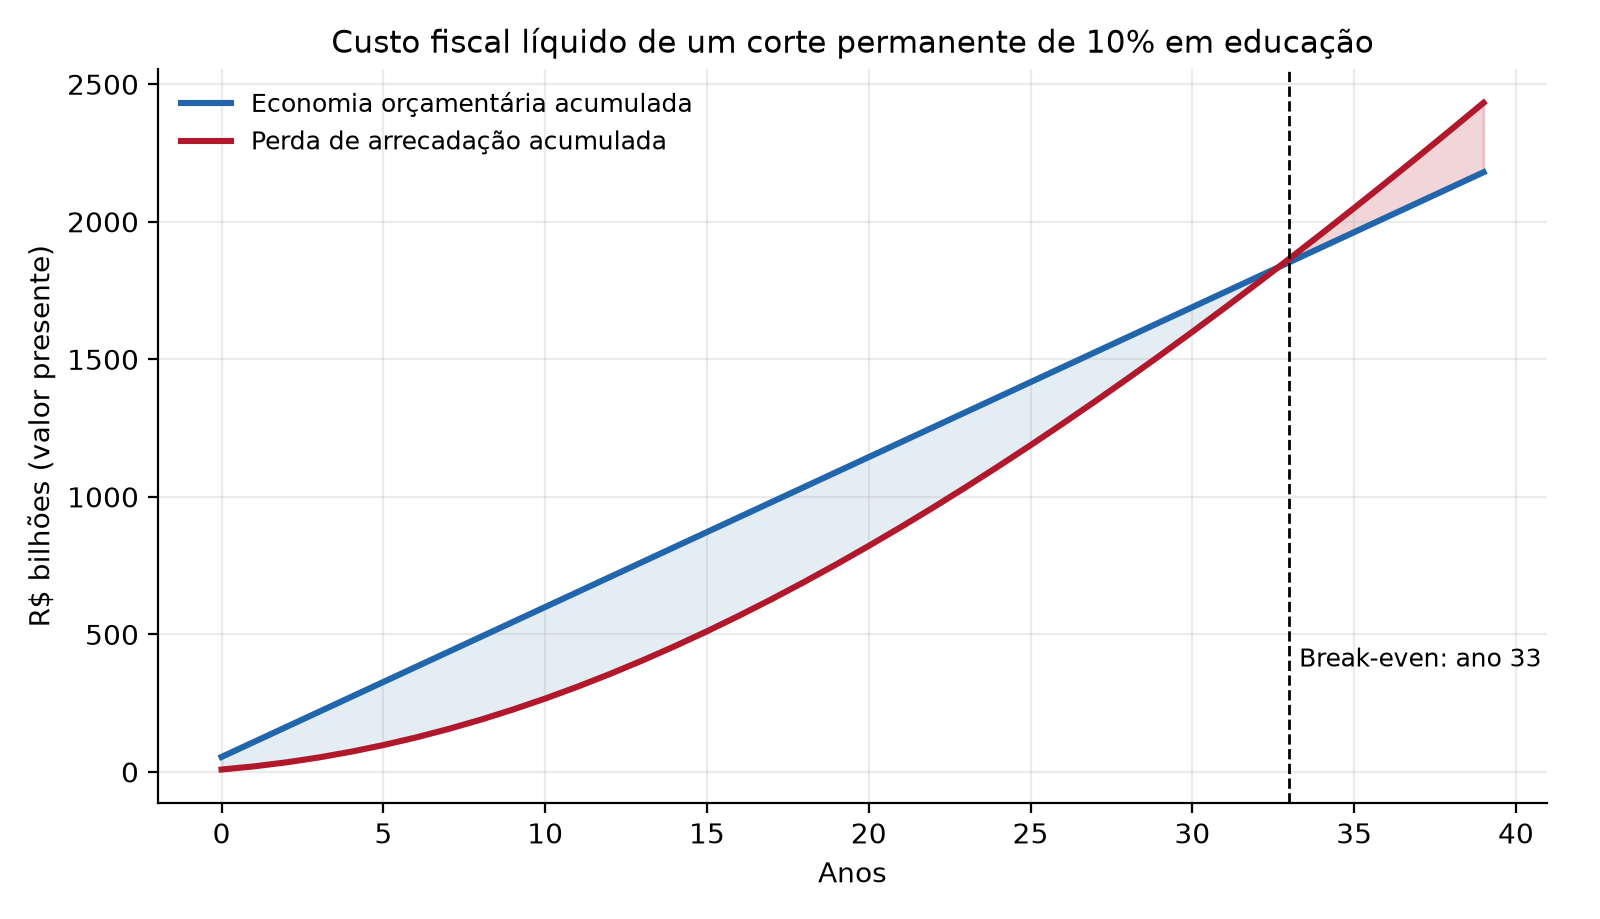
\includegraphics[width=\textwidth]{figures/custo_fiscal.png}
\end{minipage}\hfill
\begin{minipage}{0.43\textwidth}\centering
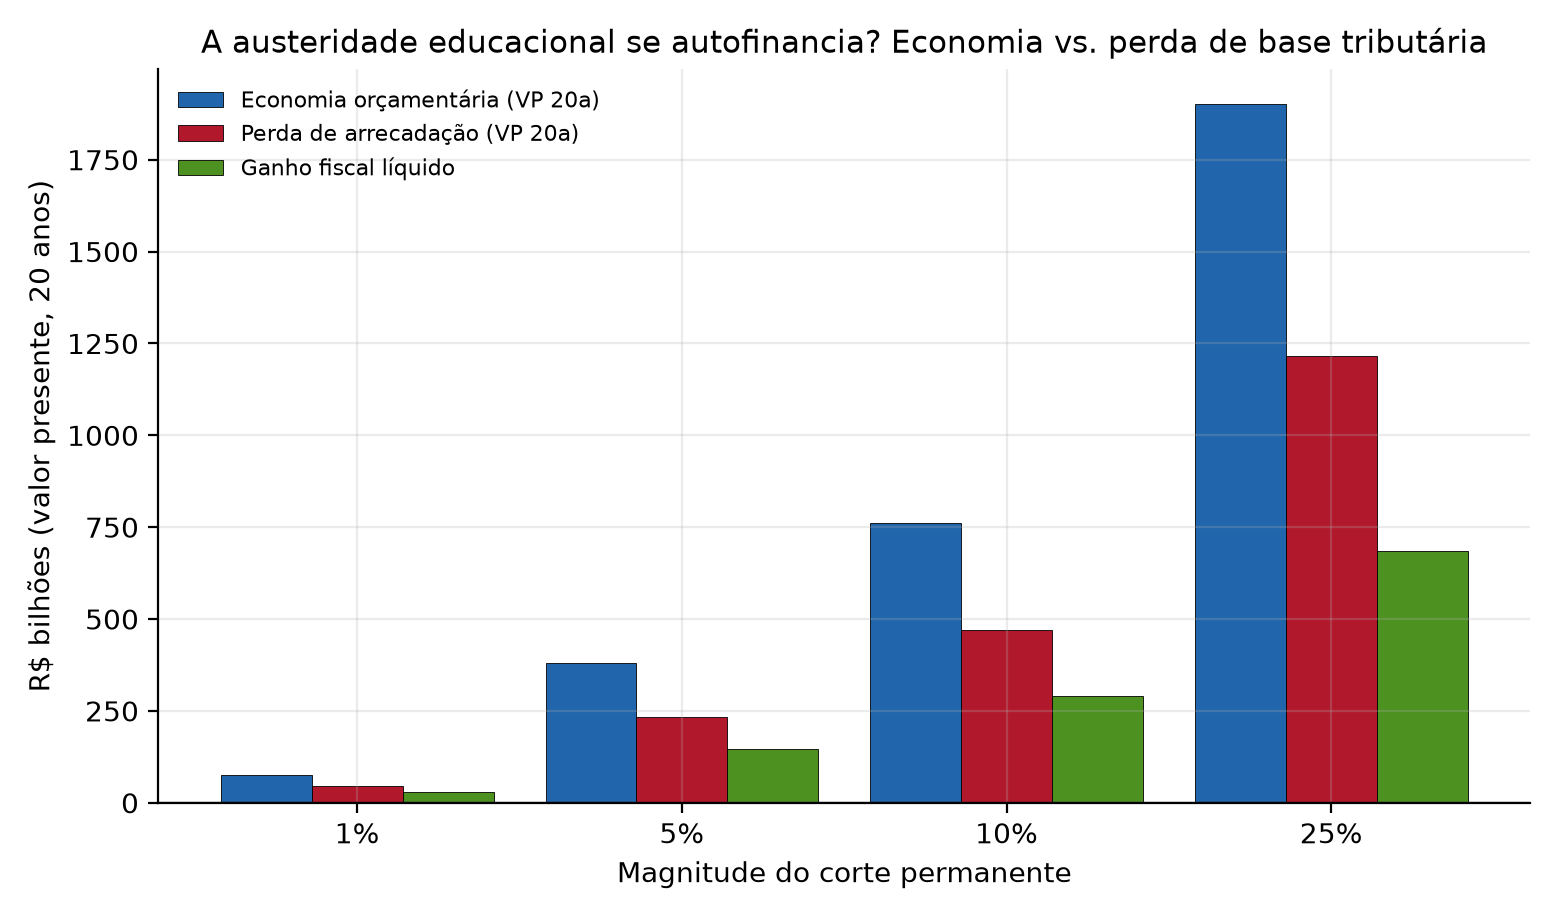
\includegraphics[width=\textwidth]{figures/custo_fiscal_barras.png}
\end{minipage}
\caption{Custo fiscal l\'iquido no tempo (corte de $10\%$, esq.) e economia \emph{vs.}\ perda de arrecada\c{c}\~ao por magnitude (VP 20 anos, dir.)}
\label{fig:fiscal}
\fonte{Elabora\c{c}\~ao pr\'opria.}
\end{figure}

% =============================================================================
\section{Bem-estar e multiplicadores}\label{sec:bemestar}
% AUTHOR WRITES
% =============================================================================

\begin{figure}[H]
\centering
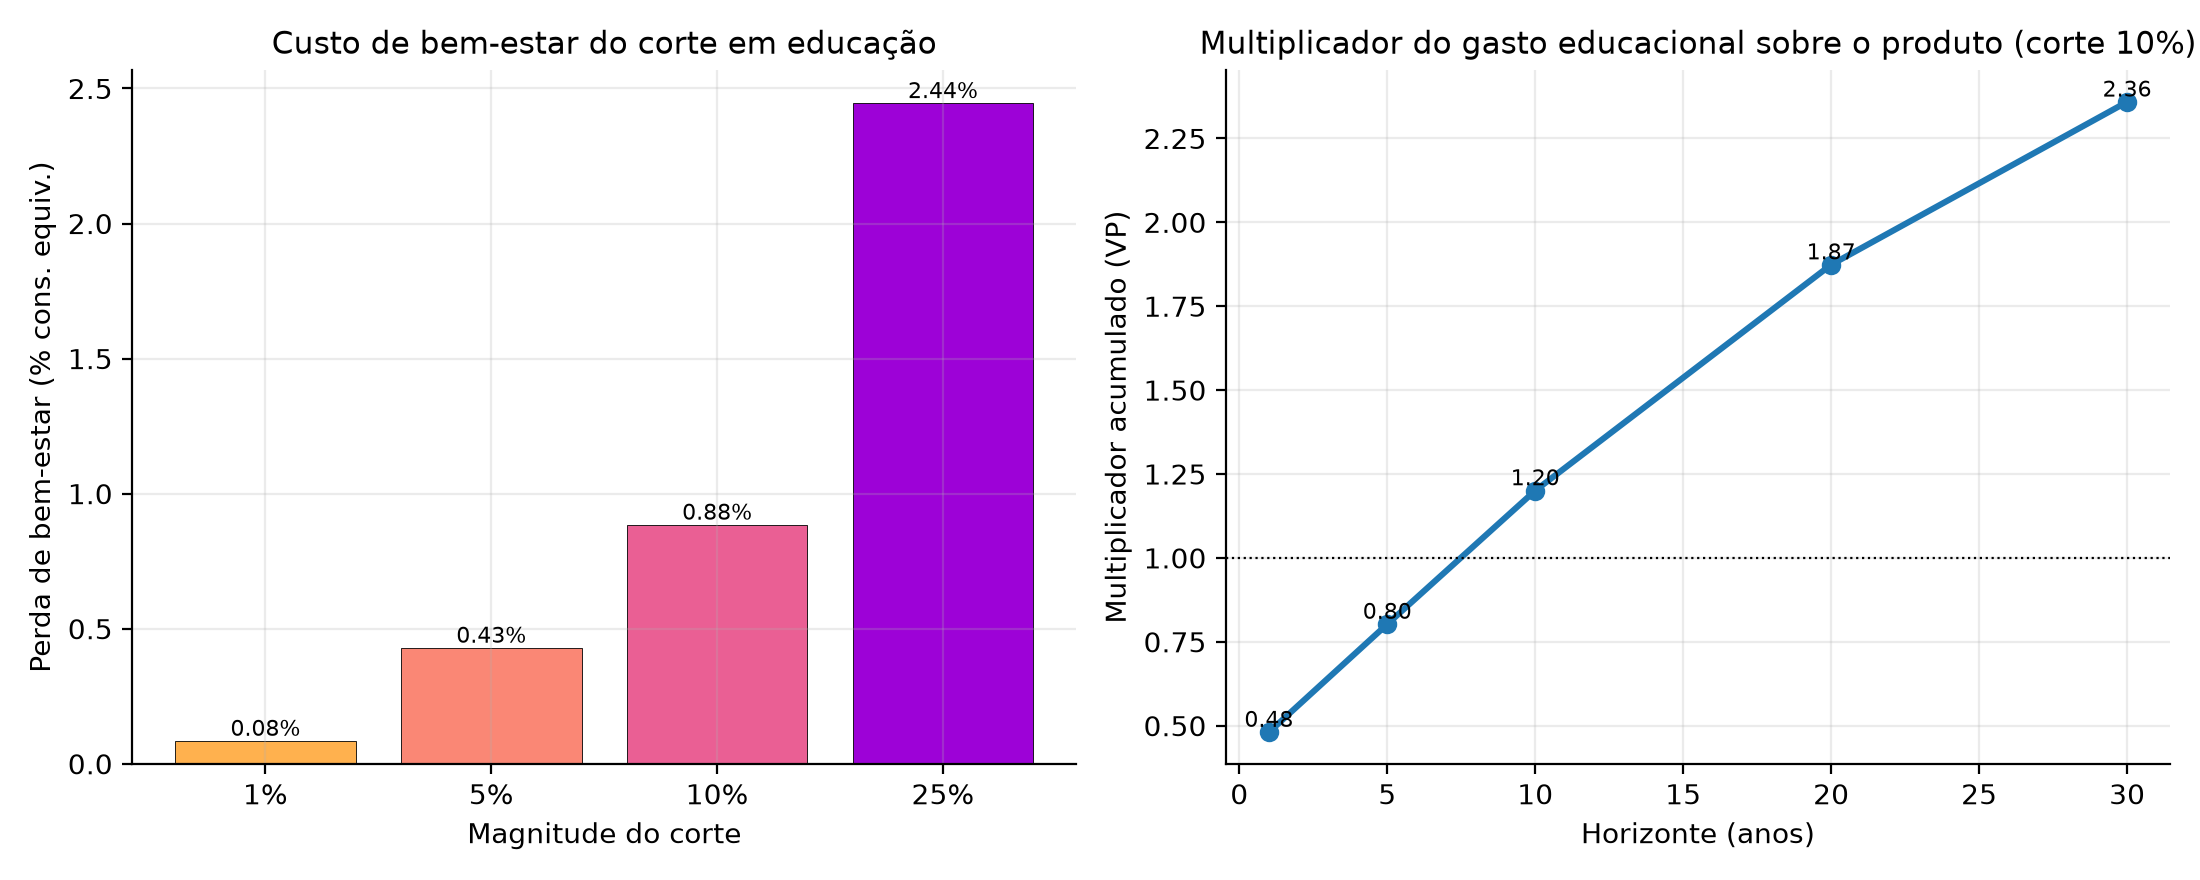
\includegraphics[width=\textwidth]{figures/bemestar_multiplicador.png}
\caption{Perda de bem-estar em equivalente de consumo (esq.) e multiplicador acumulado do gasto educacional (dir.)}
\label{fig:bemestar}
\fonte{Elabora\c{c}\~ao pr\'opria.}
\end{figure}

\begin{table}[H]
\centering
\caption{Multiplicador do gasto educacional sobre o produto (por horizonte)}
\label{tab:mult}
\small
\begin{tabular}{lrrrrrr}
\toprule
Corte & Impacto & Cum.\ 1a & Cum.\ 5a & Cum.\ 10a & Cum.\ 20a & Cum.\ 30a \\
\midrule
1\% & 0,49 & 0,49 & 0,80 & 1,19 & 1,84 & 2,31 \\
5\% & 0,48 & 0,48 & 0,80 & 1,19 & 1,85 & 2,33 \\
10\% & 0,48 & 0,48 & 0,80 & 1,20 & 1,87 & 2,36 \\
25\% & 0,47 & 0,47 & 0,81 & 1,23 & 1,94 & 2,45 \\
\bottomrule
\end{tabular}

\begin{minipage}{0.9\textwidth}\vspace{2pt}\scriptsize
Nota: multiplicador de impacto = $\Delta Y_0/\Delta G^e_0$; acumulado de $n$ anos = raz\~ao entre valores presentes de $\Delta Y$ e $\Delta G^e$ at\'e $n$.
\end{minipage}
\fonte{Elabora\c{c}\~ao pr\'opria.}
\end{table}

% =============================================================================
\section{Incid\^encia regional e desigualdade}\label{sec:regional}
% AUTHOR WRITES
% =============================================================================

\begin{figure}[H]
\centering
\begin{minipage}{0.56\textwidth}\centering
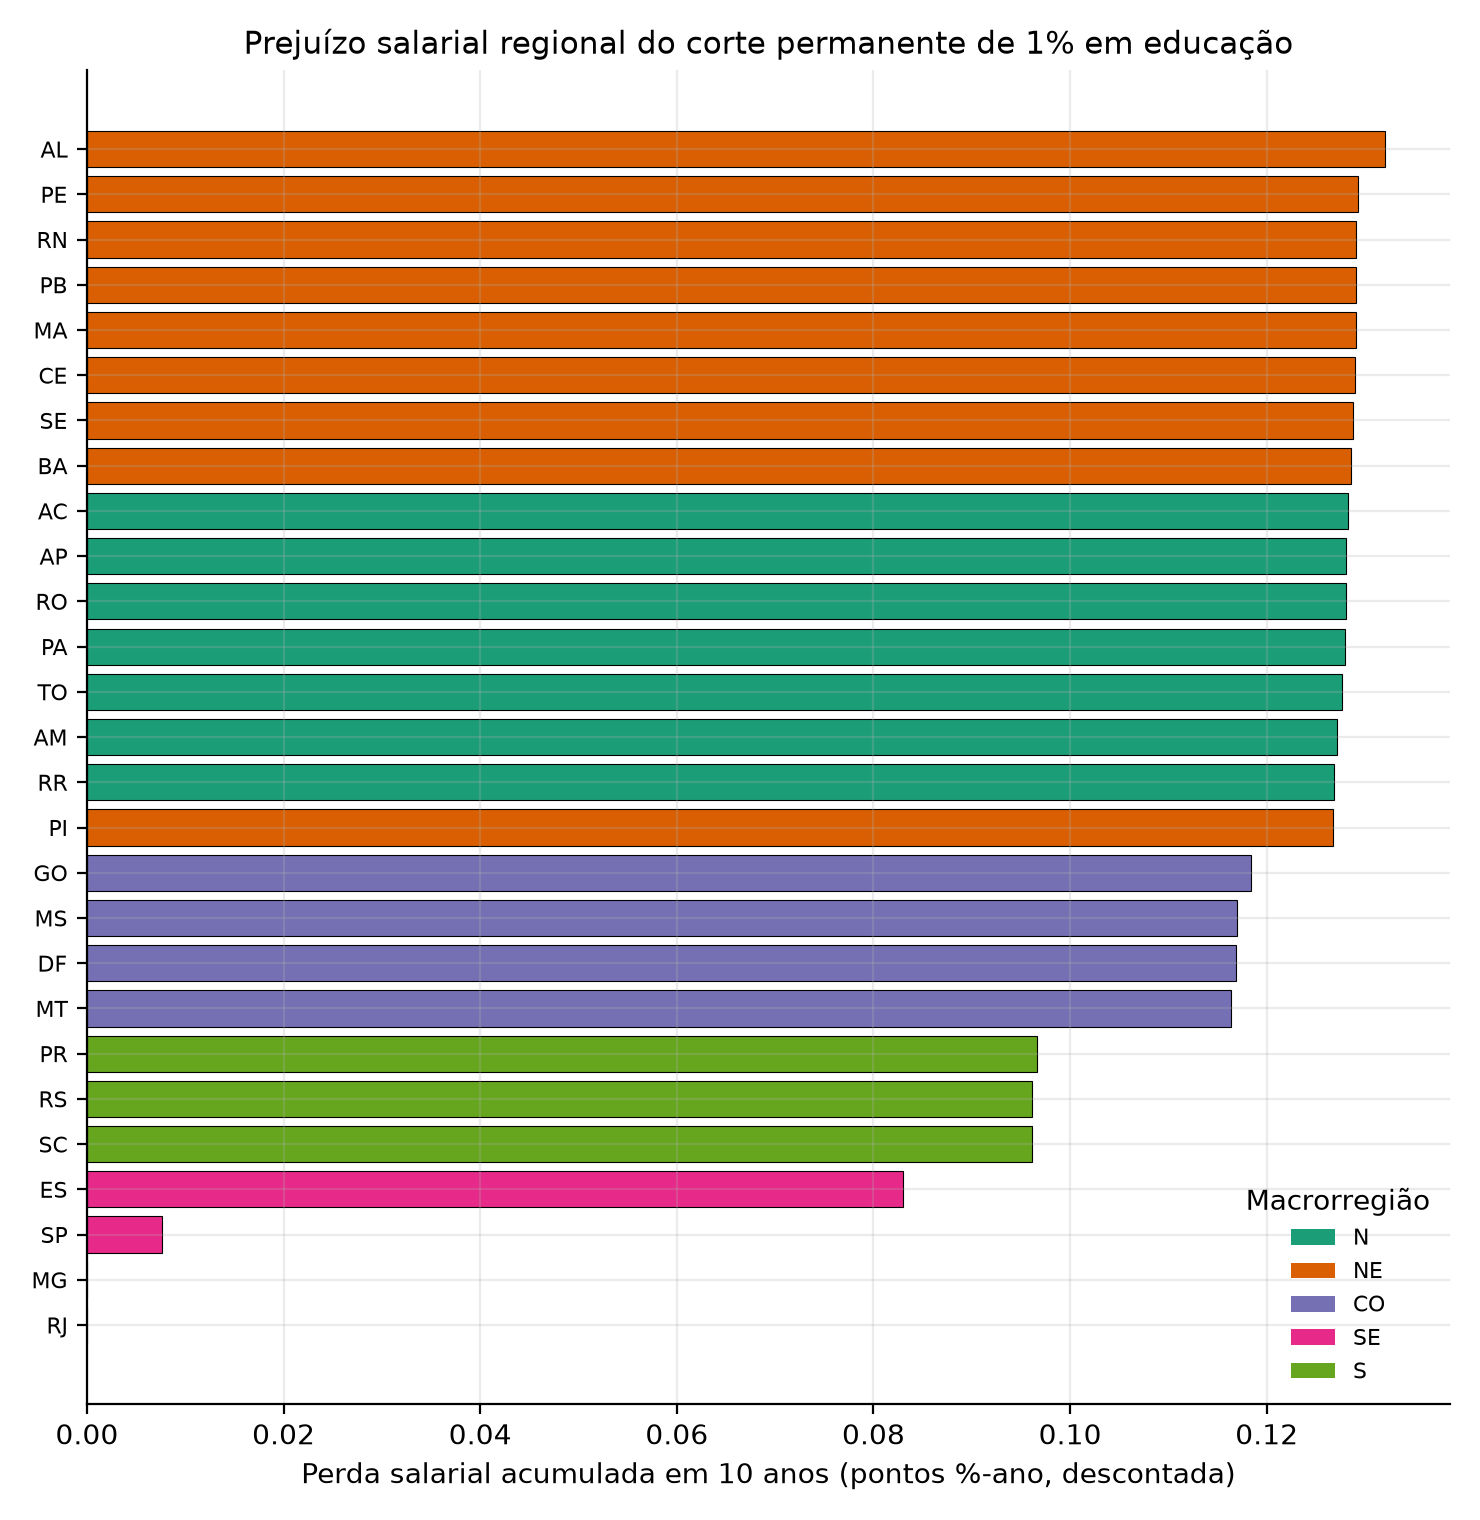
\includegraphics[width=\textwidth]{figures/projecao_regional.png}
\end{minipage}\hfill
\begin{minipage}{0.42\textwidth}\centering
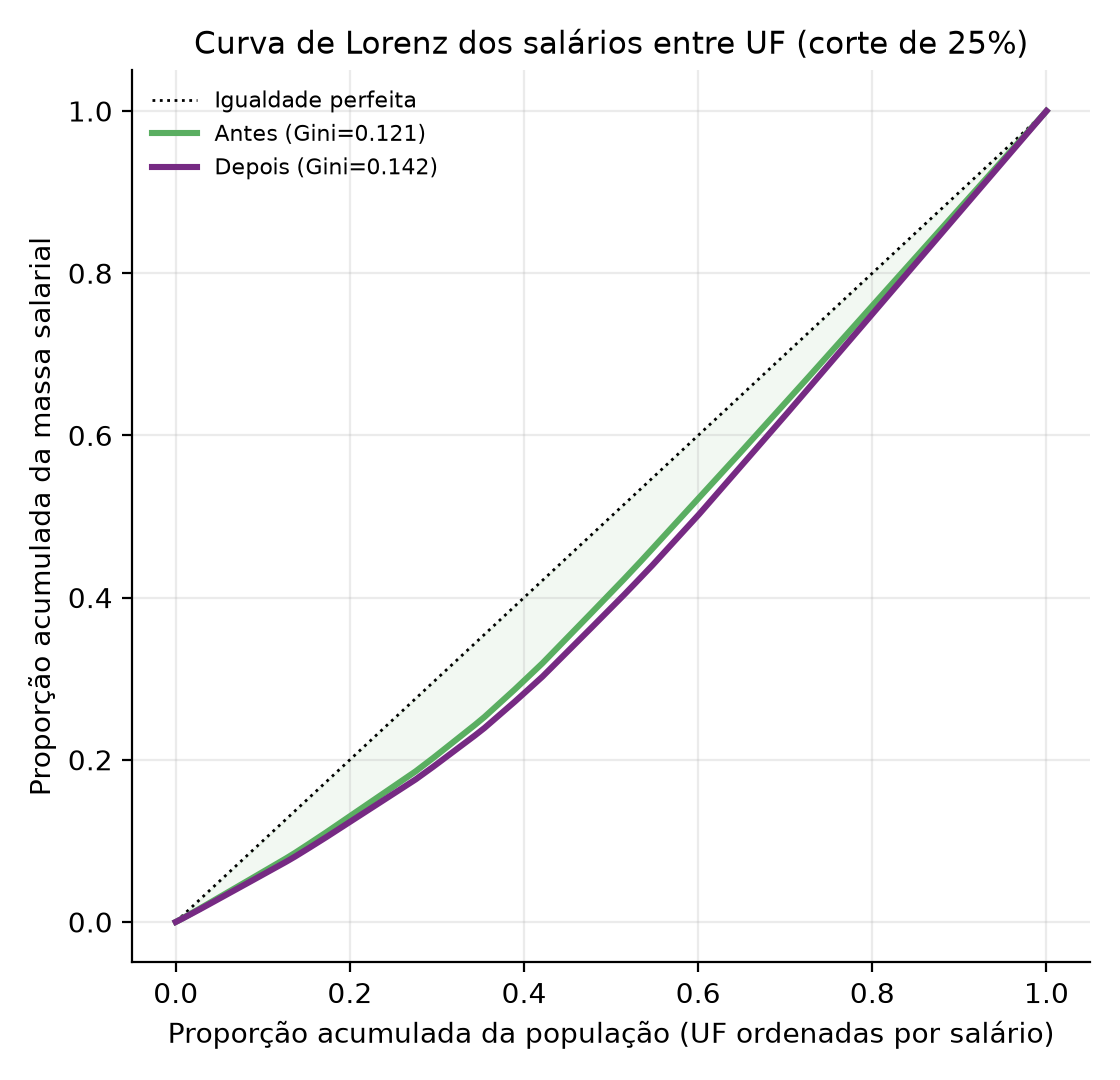
\includegraphics[width=\textwidth]{figures/lorenz.png}
\end{minipage}
\caption{Perda salarial acumulada (10 anos) por UF do corte de $1\%$ (esq.) e curva de Lorenz dos sal\'arios entre UF, antes e depois do corte de $25\%$ (dir.)}
\label{fig:proj}
\fonte{Combina\c{c}\~ao da IRF salarial do DSGE com elasticidades regionais encolhidas.}
\end{figure}

\begin{figure}[H]
\centering
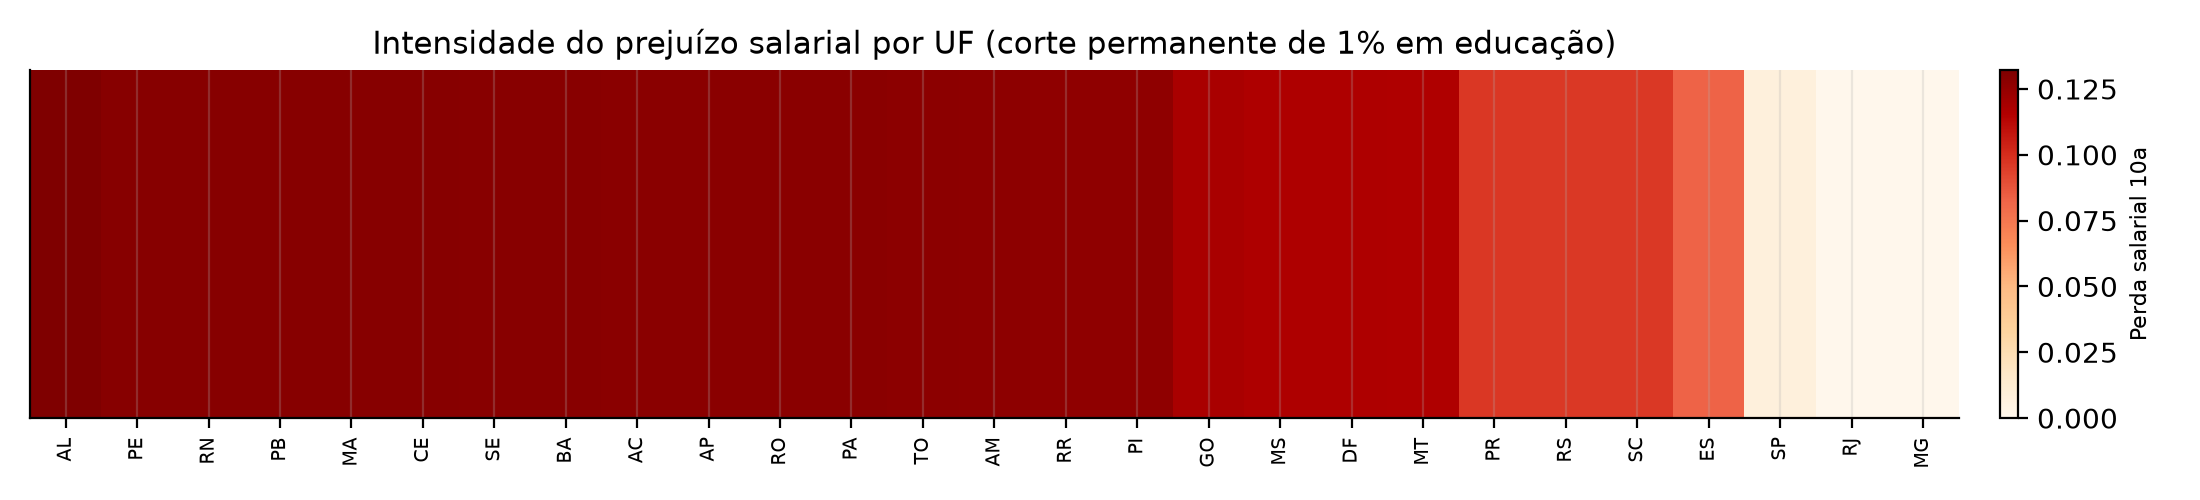
\includegraphics[width=\textwidth]{figures/mapa_calor_uf.png}
\caption{Intensidade do preju\'izo salarial por UF}
\label{fig:mapa}
\fonte{Elabora\c{c}\~ao pr\'opria.}
\end{figure}

\begin{figure}[H]
\centering
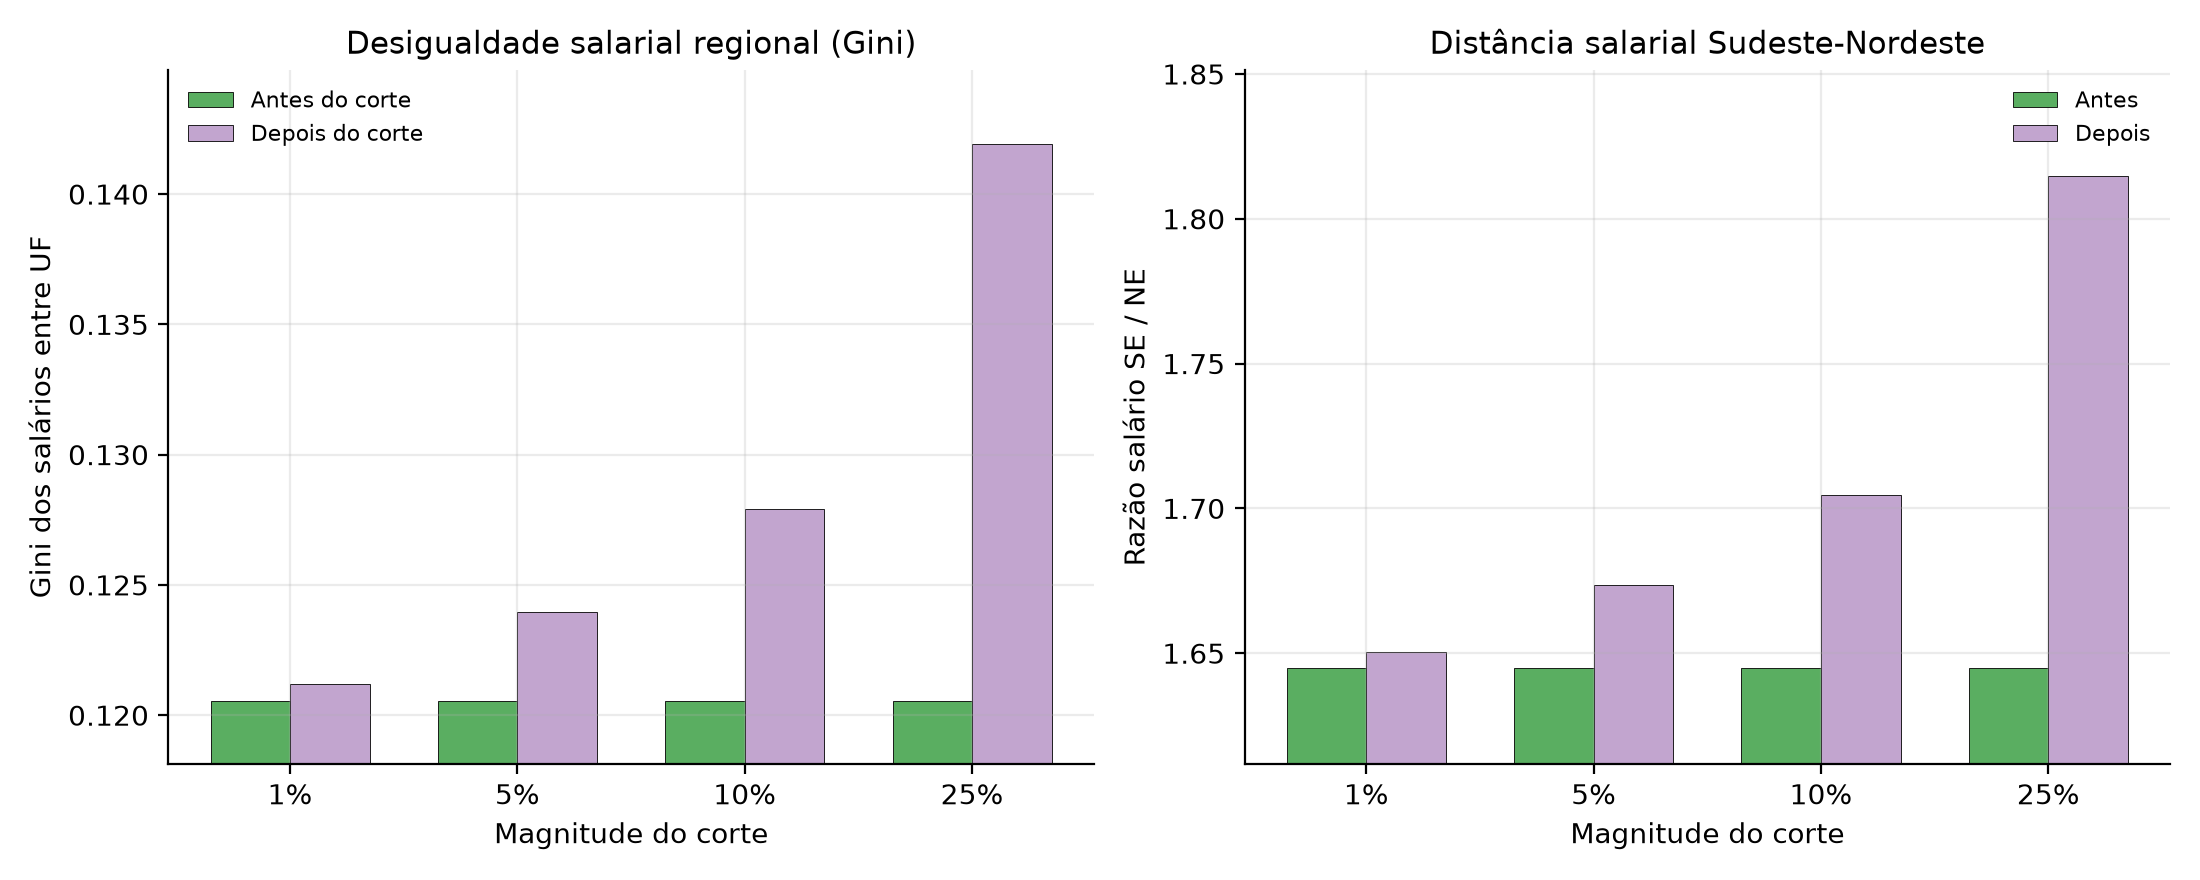
\includegraphics[width=\textwidth]{figures/desigualdade_gini.png}
\caption{Desigualdade salarial regional antes e depois do corte: Gini entre UF (esq.) e raz\~ao Sudeste/Nordeste (dir.)}
\label{fig:gini}
\fonte{Elabora\c{c}\~ao pr\'opria.}
\end{figure}

\begin{table}[H]
\centering
\caption{Desigualdade regional por magnitude do corte}
\label{tab:desig}
\small
\begin{tabular}{lrrrrr}
\toprule
Corte & Gini antes & Gini depois & $\Delta$ Gini (\%) & SE/NE antes & SE/NE depois \\
\midrule
1\% & 0,1205 & 0,1212 & 0,53 & 1,645 & 1,650 \\
5\% & 0,1205 & 0,1240 & 2,83 & 1,645 & 1,674 \\
10\% & 0,1205 & 0,1279 & 6,10 & 1,645 & 1,705 \\
25\% & 0,1205 & 0,1419 & 17,72 & 1,645 & 1,815 \\
\bottomrule
\end{tabular}

\begin{minipage}{0.9\textwidth}\vspace{2pt}\scriptsize
Nota: Gini e raz\~ao SE/NE dos sal\'arios m\'edios entre UF, ponderados pela popula\c{c}\~ao (Censo 2022), antes e depois do choque permanente.
\end{minipage}
\fonte{Elabora\c{c}\~ao pr\'opria.}
\end{table}

\begin{table}[H]
\centering
\caption{Estados com maior perda salarial projetada (12 maiores)}
\label{tab:proj}
\small
\begin{tabular}{llrrr}
\toprule
UF & Região & Elast.\ EB & Perda sal.\ 10a & Perda sal.\ 20a \\
\midrule
AL & NE & 0,212 & 0,132 & 0,765 \\
PE & NE & 0,208 & 0,129 & 0,749 \\
RN & NE & 0,208 & 0,129 & 0,748 \\
PB & NE & 0,208 & 0,129 & 0,748 \\
MA & NE & 0,208 & 0,129 & 0,748 \\
CE & NE & 0,207 & 0,129 & 0,748 \\
SE & NE & 0,207 & 0,129 & 0,746 \\
BA & NE & 0,207 & 0,129 & 0,745 \\
AC & N & 0,206 & 0,128 & 0,744 \\
AP & N & 0,206 & 0,128 & 0,742 \\
RO & N & 0,206 & 0,128 & 0,742 \\
PA & N & 0,206 & 0,128 & 0,742 \\
\bottomrule
\end{tabular}

\fonte{Elabora\c{c}\~ao pr\'opria.}
\end{table}

% =============================================================================
\section{Discuss\~ao}
% AUTHOR WRITES
% =============================================================================

% =============================================================================
\section{An\'alise de robustez}
% AUTHOR WRITES
% =============================================================================

% =============================================================================
\section{Limita\c{c}\~oes e agenda emp\'irica definitiva}\label{sec:agenda}
% AUTHOR WRITES
% =============================================================================

% =============================================================================
\section{Conclus\~ao}
% AUTHOR WRITES
% =============================================================================

% =============================================================================
\bibliography{referencias}
\appendix
\section{Deriva\c{c}\~ao das condi\c{c}\~oes de equil\'ibrio}\label{ap:deriv}
% AUTHOR WRITES
% =============================================================================

\section{Estado estacion\'ario e EE terminal end\'ogeno}\label{ap:ss}
% AUTHOR WRITES

\section{Elasticidades estaduais}\label{ap:elast}
% AUTHOR WRITES
\begin{table}[H]
\centering
\caption{Elasticidade sal\'ario-educa\c{c}\~ao por UF: bruta (\emph{bootstrap}) e encolhida (EB)}
\label{tab:elastuf}
\scriptsize
\begin{tabular}{llrrrcr}
\toprule
UF & Reg. & Elast. & IC inf. & IC sup. & Sig.\,95\% & Elast. EB \\
\midrule
AL & NE & 0.441 & 0.335 & 0.609 & Sim & 0.212 \\
GO & CO & 0.352 & 0.152 & 0.488 & Sim & 0.190 \\
AC & N & 0.315 & 0.159 & 0.680 & Sim & 0.206 \\
AP & N & 0.249 & -0.022 & 0.462 & -- & 0.206 \\
PE & NE & 0.235 & 0.044 & 0.507 & Sim & 0.208 \\
RO & N & 0.234 & 0.008 & 0.420 & Sim & 0.206 \\
PA & N & 0.232 & -0.083 & 0.526 & -- & 0.206 \\
RN & NE & 0.204 & -0.033 & 0.442 & -- & 0.208 \\
PB & NE & 0.193 & -0.197 & 0.692 & -- & 0.208 \\
PR & S & 0.181 & 0.069 & 0.298 & Sim & 0.155 \\
MA & NE & 0.180 & -0.367 & 0.604 & -- & 0.208 \\
TO & N & 0.172 & 0.004 & 0.345 & Sim & 0.205 \\
MS & CO & 0.169 & -0.067 & 0.531 & -- & 0.188 \\
RS & S & 0.155 & 0.017 & 0.384 & Sim & 0.155 \\
ES & SE & 0.152 & 0.082 & 0.251 & Sim & 0.133 \\
SC & S & 0.138 & -0.181 & 0.578 & -- & 0.155 \\
DF & CO & 0.133 & -0.447 & 0.368 & -- & 0.188 \\
AM & N & 0.130 & -0.040 & 0.277 & -- & 0.205 \\
CE & NE & 0.121 & -0.276 & 0.438 & -- & 0.207 \\
SE & NE & 0.120 & -0.147 & 0.322 & -- & 0.207 \\
MT & CO & 0.092 & -0.110 & 0.285 & -- & 0.187 \\
SP & SE & 0.062 & -0.286 & 0.430 & -- & 0.012 \\
BA & NE & 0.060 & -0.205 & 0.271 & -- & 0.207 \\
RR & N & 0.038 & -0.149 & 0.241 & -- & 0.204 \\
PI & NE & -0.032 & -0.201 & 0.107 & -- & 0.204 \\
RJ & SE & -0.156 & -0.339 & 0.037 & -- & 0.000 \\
MG & SE & -0.201 & -0.393 & 0.070 & -- & 0.000 \\
\bottomrule
\end{tabular}

\fonte{Elabora\c{c}\~ao pr\'opria a partir de 2.000 reamostragens.}
\end{table}

\section{Reprodutibilidade}\label{ap:repro}
% AUTHOR WRITES

\end{document}
